\documentclass[a4paper]{article}

\usepackage{amsmath}  % extra math features
\usepackage{booktabs}  % nice tables
\usepackage[margin=25mm]{geometry}
\usepackage{graphicx} % required for inserting images
\usepackage{hyperref} % clickable hyperlinks
\usepackage{multirow}  % pandas to_latex() uses this
\usepackage{siunitx}  % use for all units
\usepackage{subcaption}  % for subfigures

% hyperref settings for better looking links
\hypersetup{
  colorlinks=true,
  linkcolor=blue,
  urlcolor=blue,
}

% NOTE : Use as \si{\kph} or \si{\mps}
\def\kph{\kilo\meter\per\hour}
\def\mps{\meter\per\second}
    
\title{
  DRAFT: v2 \\
  Vibration Characterisation of Strollers and\\
  Cargo Bicycles for Transporting Infants\\
  \vspace{2mm}
  \large{Prepared for VeiligheidNL}
}
% Gabriele as first, Jason as last, alphabetical for intermediate (discuss in meeting if other method desired
\author{
Gabriele Dell'Orto \and
Brecht Daams \and
Riender Happee \and
Arjo J. Loeve \and
Jesper Meijerink \and
Georgios Papaioannou \and
Thomas Valk \and
Jason K. Moore
}

\begin{document}

\maketitle

\section*{\centering Notice}
%
\textbf{This is a draft report. The values and results must be considered preliminary and may change as the analysis is refined and rechecked.}

\begin{abstract}
    TODO
\end{abstract}

\section{Introduction}
%
% Paragraph about motivation 
Cycling, one of the active transportation modes is advantageous for health~\cite{Oja1998} and greatly contributes to reducing CO2 emissions, congestion, and air
pollution ~\cite{Neves2019}.
As a result, bikes have been widely used as a mean to deliver goods to consumers, and also for daily commuting to work and personal matters (shopping, commuting with children/infants, and others).
Among all journeys in EU, 20-40$\%$ are by bike or on foot, with bicycle trips being most frequent in the Netherlands, Denmark and Sweden and less frequent in Finland.
Various countries and employers provide incentives to increase the use of bikes.
Nevertheless, there are great challenges that need to be overcome to secure the wide acceptance and use of active transportation modes.
One of these challenges is the comfort levels experienced by riders and passengers (i.e., infants/children in cargo bikes), which is a multi-faceted aspect \cite{ayachi2015identifying} and critical for the wide acceptance and use of bikes as a daily mean of transport.

% Paragraph about comfort in bikes
Comfort on bicycles \cite{too1990biomechanics} is mostly affected by physical comfort and the impact of environmental factors (weather, route geometry and road roughness).  
Physical comfort is related with mechanical (bicycle and components design), biomechanical (whole-body vibrations, human body dynamics and kinematics) and physiological factors (individual characteristics, e.g. sex, body size, weight and others).
While there is extensive literature exploring the impact of environmental factors (i.e., irregular road surface quality, weather conditions) on cyclists' comfort \cite{Stinson2003,Hagemeister2003,ayachi2015identifying,Verhoeven2017,Teixeira2020}, there is limited work on understanding the biomechanical and physiological factors of comfort while riding a bike or being driven by a bike (infants/children on cargo bikes or trailers).
In this paper, we will explore biomechanical comfort, by assessing the whole-body vibrations that could be experienced by transported infants, and evaluating potential health risks and discomfort that might arise.

% Paragraph about transmission of vibrations
Biomechanical comfort is mostly related to the vibrations induced by road irregularities and transmitted via the vehicle to the human body and head while being driven. 
According to the literature, the road irregularities are a critical factor for the amplitude of the resulting vibrations experienced by the bicyclists and passengers, as the vibrations induced on the body and head are not efficiently isolated due to the lack of suspension systems in most of the bike models \cite{vasudevan2017comparison}.
The bike design and its specific configuration can affect the sitting posture, and eventually the transmissibility of the vibrations \cite{Brand2020,Verma2016}.
The sitting posture can also vary in case of children/infants who may be transported sitting or lying down in a different--than the bicyclist--location (e.g. above a wheel when in a bike seat) and in/on a different ‘seat’ (a car seat, bike seat, stroller seat or cot). 
These all influence the level of whole-body vibrations and the transmission of the vibrations from the seat to the body and head. 
Furthermore, the amplitude of the vibrations experienced by bicyclists/passengers while biking or being transported may increase because of increased travelling speed either due to running with a stroller or due to the increased power offered by electric bikes (with and without trailers), and cargo bikes.
The average speed of electric bikes and speed pedelecs is 19$\%$ higher (21,0 km/h) and up to 63$\%$ higher (28,1 km/h), respectively, than the average speed of conventional bicycling (SWOV, 2022, p. 8).
The intensity of these vibrations could become even more critical with the change of load, which could be related with age and size of the infant/children transported. 
However, there is limited literature exploring the whole-body vibrations of infants and children being transported by bikes with trailers, cargo bikes or even cots \cite{Schwanitz2020,MalteChildComfort2022}.

% Paragraph about children in bikes
% 
One of the research fields closely related to vibrations acting on infants during transportation is that of inflicted head injury by shaking trauma (IHI-ST) (Vester, 2019; Zandwijk, 2019; Hutchinson, 2024). 
However, there is a lack of reliable, applicable, validated injury thresholds for assessing IHI-ST risks and hardly any chance that these thresholds do apply to vibration studies.
Similarly, even if there are significant indications that the vibration amplitude affects comfort in bikes or strollers, there are no standard assessment methods or guidelines available with regards to their design. 
ISO 2631, the international standard for assessing whole-body vibrations, was derived using datasets on motion platforms, adults as human participants and sitting postures which are adopted in passenger vehicles rather than in bikes.
This inconsistency was captured by Gao et al. (2018), who derived different limits of comfort for adults compared to ISO-2631.
In addition, the exposure time to the vibrations is not considered as a factor of comfort by the ISO2631, despite having a clear impact on health risks according to the European Directive (2002/44/EC, 2002).

% Paragraph Potential effects of vibrations on adults
Despite the lack of clarity with regards to comfort assessment or inflicted head injury by shaking trauma for children/infants on bikes, there are clear indications in the literature that these should be explored. 
About 36$\%$ of males and 42$\%$ of females in the total sample of 900 people (Groenendijk et al., 1992) had various complaints about comfort.
Discomfort for both men and women occurred even during short bicycle trips (3—10 km). 
Duarte et al. (2018) considered four different exposure durations and concluded that their results rejected the hypothesis that the exposure duration or the vibration dose value (VDV) by itself are important parameters on the vibration influence.
Furthermore, cyclists can avoid or reduce shocks and uncomfortable vibrations for a short time by standing on the pedals, which can increase comfort in some situations. 
This is an option that children sitting or lying in transportation systems do not have.
Results from research into comfort of adult cyclists are assumed to be children sitting or lying in transportation systems, leading potentially to misinterpretations. 
Hence, there is a need to re-focus on the impact of vibrations on infants and children health and comfort \cite{rybarczyk2020physiological} to secure the safe, comfortable and wide use of bikes. 

Schwanitz et al. (2020a and 2020b) measured seat pan accelerations of a child bicycle trailer with anthropomorphic children shaped sandbag dummies (baby and toddler sizes) present in the seats. 
They report ISO 2631-1 weighted RMS vertical accelerations riding over smooth asphalt, gravel, and cobblestones. 
Tire pressure and the number of passengers had no significant effect on vibration magnitude, but road surface and travel speed did. 
The baby sized dummy (5 kg) experienced 20$\%$ higher vibration than the toddler sized dummy (10 kg). 
They express that their measured values generally exceed the ISO 2631-1 occupational norms for 4-8 hour vibrational comfort of adults.

Kayna-Forster (2020) measured acceleration in bicycle child trailers with human subjects aged 12 months to 6 years over asphalt and gravel terrain. 
The bicyclists travelled at their chosen comfort speeds and averaged 12 km/h over the 20 minute ride duration. According to the assessment using ISO-2631 and the use of an unspecified correction, the vibrations are similar to the ones experienced in car seats in vehicles and illustrated moderate or low health risk for a 2 hour duration. 
On the other hand, the uncorrected values point to moderate and high risks, which align with subsequent studies detailed below.
As expected, she also pointed out that cargo trailers with suspension systems did exhibit lower seat accelerations. 
Her second study utilised a laboratory vibration excitation system, similar to Ota et al. (2012) to determine the impact of independent variables (terrain type, trailer type, and cushion type) to the dependent variable vibration magnitude at the interface between the trailer seat and dummy buttock of a child. 
Terrain type had the greatest influence on vibration exposure levels followed by trailer type (p<0,001). 
Adding gel cushions did not significantly influence vibration measured at the seat/buttock interface.

 
Whole-body vibration by means of vibration total values obtained at toddler and baby dummy in dependence on different road surfaces, load cases, tire pressures, and velocities. Vibration discomfort threshold value 2.0 m/s2 is indicated with a dashed line. (Schwanitz et al., 2020a)
Liu (2023) developed a benchtop vibration excitation system for a unsuspended bicycle trailer capable of applying controlled and simulated road vibrations to the trailer. They measured IS0 2631-1 weighted RMS vertical accelerations at the seat pan ranging from 2,8 to 3,6 m/s2 for seat masses of 0 kg to 23 kg. Vibration increased with load at a high tire pressure (150 kPa) and had less variation at a lower pressure (75 kPa). They point out that these values are rated as “extremely uncomfortable” as per the 4-8 hour ISO 2631-1 occupational norms.
Rothhämel (2023) found ISO 2631-1 weighted RMS child trailer seat pan acceleration between 1 and 5 m/s2 for speeds between 10 and 20 km/h on smooth asphalt with large tire pressure variations having small effects. On cobblestones this range increased to 2 to 9 m/s2 for the same speed range. The child trailer exhibited larger weighted RMS vibration than a tadpole configuration three-wheel cargo bicycle with the child seat between the front wheels. Both the trailer and cargo bicycle child seats had generally larger magnitude vibrations than experienced in an automobile seat travelling at 30 km/h on a rough road (~3 m/s2) (Gromadowski 2013).
Rothhämel and Liu (2023) made improvements to the work by Lui (2023). They used the benchtop excitation device and the bicycle trailer with a 6,5 kg mass representing an infant and measured seat pan vertical acceleration at 2047 Hz sampling rate with excitation bandwidth of 17 Hz. They report ISO 2631-1 weighted vertical RMS ranging from 3 to 5 m/s2 for tire pressures from 50 to 400 kPa, which are higher value accelerations than reported by Liu (2023), See Figure 16. These values also fall into the “extremely uncomfortable” zone for the ISO 2631-1 4-8 hour occupational norms.




This paper reports on the vibration induced on infants of different ages when transported in strollers and cargo bicycles. 
Vibration can be related to discomfort and might lead to negative health consequences.  
In fact, vibrations induced by such transportation means have brought up as alternative scenarios in court cases concerning suspicion of infant injuries inflicted by violent shaking, such as in a recent case about a twin in 2023 in the Netherlands.
However, the topic is poorly addressed in scientific literature, and only a few studies focus on the effect of vibration on babies. 
To measure the actual vibration transmitted to the babies, we equipped five strollers and two cargo bicycles with inertial measurement units (IMU) and conducted several experiments on different road surfaces and travel speeds,
using dummies representing the size and mass of 0, 3, and 9 months old infants.
We present results in the time and frequency domains,
which allows comparing vertical accelerations at the baby-seat interface, as
recommended by ISO-2631-1 norms for vibration discomfort. 
We investigated the influence of different variables on vibration, such as type of vehicle, baby seat, travelling speed, dummy size and mass, and road surfaces.

\section{Methods}
%
\subsection{Experimental Methodology}
%
\subsubsection{Test Equipment}
%
Vibration measurements were conducted at approximate constant speed using five
different strollers, two cargo bicycles, and two baby seats, chosen for their
popularity and/or distinctive features:

\paragraph{Strollers}
%
\begin{description}
  \item[Maxi-Cosi Street Plus] Among the most popular brands, this stroller comes
  with a cot configuration (0-3 months) and a baby seat option. It has large
  wheels, with only a marginal suspension system.
  (\href{https://www.maxi-cosi.nl/kinderwagens/street-plus?color_swatch_id=5519}{Maxi-cosi website})
  \item[Stokke BABYZEN YOYO 0+] The smallest foldable stroller on the
  market. It has only a marginal suspension system and smaller wheels compared
  to the other strollers on the market. 
  (\href{https://tinylibrary.nl/products/kinderwagen-babyzen-yoyo-0-plus}{Model
  rented for the experiment})
  \item[Bugaboo Fox 5] Featured by large wheels and a suspension system
  that makes it an all-terrain stroller according to the manufacturer. It has
  a large puncture-proof tyres and an air-permeable mattress.
  (\href{https://www.bugaboo.com/nl-nl/speciale-aanbiedingen/bugaboo-fox-5-bassinet-and-seat-stroller-black-base-midnight-black-fabrics-midnight-black-sun-canopy-PV006272.html?gad_source=1&gclid=Cj0KCQiA1Km7BhC9ARIsAFZfEIuB-6fQPRl5KyIHVJtion5lyD_Z1Qn-IP3shWoB_HXFozM1ySTXNfgaAgzFEALw_wcB&gclsrc=aw.ds}{Bugaboo
  website})
\end{description}

\paragraph{Cargo Bicycles}
%
\begin{description}
  \item[Urban Arrow Bicycle] A popular electric cargo bicycle in The
  Netherlands. This vehicle has two inline wheels which makes it roll into curves like a regular bicycle. It is featured by a long frame that can carry
  loads usually placed in between the rider and the front wheel. 
  (\href{https://urbanarrow.com/}{Urban Arrow website})
  \item[Keiler Tricycle] A tadpole cargo tricycle (two wheels in the front, one in the
  rear) without electric assist. This vehicle will not roll into
  curves. However, differing road surface unevenness at the left and right front
  wheel will induce lateral roll and lateral acceleration in infants. We
  added masses in specific locations to simulate the presence of an electric
  motor and battery package.
 (\href{https://kashop.nl/product/keiler-bakfiets/}{Product Webpage}) 
\end{description}
  
\paragraph{Baby Seats}
%
These baby seats were mounted in the cargo bays of the two cargo bicycles.
%
\begin{description}
  \item[Maxi-Cosi X Joolz Pebble Pro i-Size Car Seat] Can be adapted to
    cargo bicycles with a fitting fixing system (e.g. ``Urban Arrow Baby Car Seat
    Adapter''). Comes with an integrated suspension system.
    (\href{https://www.maxi-cosi.nl/autostoelen/pebble-pro-i-size}{Maxi-Cosi Webpage})
  \item[Melia Baby Shell] Meant for babies from 2 to 9 months old,
    specifically designed for cargo bikes.
    (\href{https://melia.nl/product/babyschaal-4-seizoenen-comfort/}{Melia Webpage})
\end{description}
%
Appendix~\ref{app:equipment} provides figures and technical descriptions of all the strollers and cargo bicycles.

The tests involved three baby dummies with sizes and weights representative of 0, 3 and 9 months old infants. We considered the use of
``crash test dummies'' (also known as anthropomorphic test devices or ATD's) which are designed and commonly used to test
child seats in cars crash tests. However, the nearest available body
sizes for crash test dummies were a 6-weeks Q0-dummy, a 6-months Crabi dummy, and a
12-months Q-dummy. These 3 dummies are of a fundamentally different design,
hampering comparison, and do not match the desired body sizes. Moreover, these
child dummies have dynamic properties designed for crash conditions, and were designed based on
scaling of adult biomechanical data rather than child data.
Testing with real children would be unethical for the most severe conditions
tested, and would create challenges in terms of reproducibility.
Hence we bought and adapted ``reborn'' dummies available in a wide range of postures from a webshop specialising in dolls and dummies
(\href{http://www.atelier-wiesje.nl}{Atelier Wiesje}). The dummies
were filled with a mixture of cat litter sand and water to reproduce the exact weights needed for testing. Cat
litter sand features smooth and round-shaped grains, which do not
damage the dummies' materials (fabric and plastic). The weight and body height of
the dummies were made to match the are average measures for children of 0, 3 and 9 months old.
We wanted to use the measurements from Steenbekkers \cite{Steenbekkers1993}. But
the researchers provided the results only per three-month group, which did not fit our
age categories. Therefore, we decided to use the growth charts (used by clinicians to assess infant growth) to determine the average weight
and body height at the right ages. The average weight at 0 months and the
average body height at all three ages are derived from Dutch growth charts.
Measurements of Dutch children are used because these are the target group of
VeiligheidNL. Dutch children are also the tallest in Europe. The average weight
of 3 and 9 months children is derived from French growth charts. French children
are the smallest in Europe. At 3 months, the weight difference is 4 ounces and
at 9 months, it is 3 ounces compared to Dutch children.  
%
\begin{description}
  \item[Dummy 0 months] weight 3.48~\si{\kg}, size 50~\si{\cm}. Dollkit 20'',
  ``Andi Asleep'' (product code AW380008).
  (\href{http://www.atelier-wiesje.nl/index.php?item=9912---dollkit-20-_-andi-asleep--_-armen-_-_-benen----available&action=article&group_id=10000164&aid=2163&lang=NL}{Webpage})
  \item[Dummy 3 months] weight 5.90~\si{\kg}, size 62.5~\si{\cm}. Dollkit 25'',
  ``Asia - Limited Edition'' (product code 300287).
  (\href{http://www.atelier-wiesje.nl/index.php?action=article&aid=2556&group_id=10000176&lang=NL}{Webpage})
  \item[Dummy 9 months] weight 8.90~\si{\kg}. Size 70~\si{\cm}. Dollkit 28'',
  ``Hailey'' (product code 304137).
  (\href{http://www.atelier-wiesje.nl/index.php?action=article&aid=1974&group_id=10000133&lang=NL}{Webpage})
\end{description}

To achieve a realistic mass distribution in the body of the dummies, each limb was filled with a proper amount of sand. To do this, the geometry of each body segment was simplified according to pre-defined basic geometric shapes: a sphere for the head, and cylinders for the torso,
upper arms, upper legs and lower legs, according to \cite{Snyder1977}. We also assumed an equal density of each limb, and rescaled the measurements of the limb segments reported in \cite{Snyder1977} to match the dimensions of our dummies. In doing so, we were able to calculate the volume of each segment, and thus the mass of each limb of the dummies (assuming a
density of 1000~\si{\kg\per\cubic\meter}).

\subsubsection{Measurement Equipment}
%
Linear accelerations and angular velocities were measured tri-axially using Consensys Shimmer3 IMUs with a Consensys Base 6U.01 dock.
The IMUs were updated to firmware version LogAndStream v0.11.0, and
managed via the software ConsensysBASIC v1.6.0-64bit on a Dell 7310 laptop with
Microsoft Windows 10. We 3D printed supports (material: PLA) for the sensors to ensure a firm
clamp between the sensor and the bicycle/stroller tested (visible in
Figure~\ref{fig:sensors_UA}). Each vehicle was equipped with five IMUs, as
listed below. The sensors mounted on the cargo bicycle Urban Arrow
are depicted in Figure~\ref{fig:sensors_UA}. The location and orientation of the
sensors for Urban Arrow equipped with the Melia baby shell are shown in
Figure~\ref{fig:tech_drawing_UA_Melia}, both for lateral and front view.
Similarly, the Bugaboo configured to carry 0 months old infants in the baby cot is
shown in Figure~\ref{fig:tech_drawing_Bugaboo0}.
%
\begin{figure}
  \centering
  \subcaptionbox{IMU on the front fork}{\includegraphics[width=0.45\textwidth, angle=-90]{fig/FW_UA.png}}
  \subcaptionbox{IMU on the rear wheel hub}{\includegraphics[width=0.45\textwidth, angle=-90]{fig/RW_UA.png}}
  \subcaptionbox{IMU under the cargo bay}{\includegraphics[width=0.45\textwidth, angle=-90]{fig/BT_UA.png}}
  \subcaptionbox{IMUs on the baby seat surface}{\includegraphics[width=0.45\textwidth, angle=-90]{fig/Maxicosi_sensors_UA.png}}
  \caption{IMU locations on the Urban Arrow cargo bicycle. The white 3D printed
  sensor supports are visible in (a) and (c).}
  \label{fig:sensors_UA}
\end{figure}
%
\begin{figure}
  \centering
  \subcaptionbox{Lateral view}{\includegraphics[width=75mm]{fig/TechDraw_UA-Melia_lat.PNG}}
  \subcaptionbox{Front view}{\includegraphics[width=75mm]{fig/TechDraw_UA-Melia_front.PNG}}
  \caption{IMU locations on the Urban Arrow cargo bicycle, equipped with the
  Melia baby shell. Here you can see the locations from the front and the
  lateral view. All the measurements are in \si{\mm}. You can also see the
  sensors' orientation. The reference system from which we draw the measurements
  is highlighted in red and placed on the rotational axis of the front wheel.}
  \label{fig:tech_drawing_UA_Melia}
\end{figure}
%
\begin{figure}
  \centering
  \subcaptionbox{Lateral view}{\includegraphics[width=75mm]{fig/TechDraw_Bugaboo0_lat.PNG}}
  \subcaptionbox{Front view}{\includegraphics[width=75mm]{fig/TechDraw_Bugaboo0_front.PNG}}
  \caption{IMU locations on the Bugaboo Fox 5 stroller in the configuration for
  the 0 month baby. Here you can see the location from the front and the lateral
  view. All the measurements are in \si{\mm}. You can also see the sensors'
  orientation. The reference system from which we draw the measurements is
  highlighted in red, and placed on the rotational axis of the front wheel.}
  \label{fig:tech_drawing_Bugaboo0}
\end{figure}
%
\begin{enumerate}
  \item \textbf{Rear Wheel} This IMU was placed on the wheel hub (cargo
  bicycles) or clamped to the wheel (strollers) for measuring the travel speed . The travelling (longitudinal)
  speed was derived according to:
  %
  \begin{align}
    v = \omega \cdot r
    \label{eq:long-speed}
  \end{align}
  %
  where \si{\omega} is the angular speed of the wheel (obtained from the IMU's gyroscope aligned with the wheel's axis) and $r$ is the radius of the wheel.
  \item \textbf{Front Wheel} This IMU was mounted on the front wheel fork (the
  caster wheel for the stroller). This was the non-rotating measurement point closest to the
  ground. The purpose of this sensor was to measure the
  road roughness filtered out only by the tyres.  
  \item \textbf{Frame} On the cargo bicycle, an IMU was placed
  below the frontal cargo bay, clamped to the frame. This was to provide an
  understanding of the damping characteristics of the bicycle frame, together
  with an estimation of the effect of the suspension system. On the
  stroller, the IMU was placed under the baby seat.
  \item \textbf{Seat Head} IMU mounted into the baby seat, directly in
  contact with the dummy's head. This IMU measured the vibration transmitted to the
  head contact point.
  \item \textbf{Seat Buttock} This IMU was taped into the baby seat, at the
  interface between the dummy's buttock and the baby seat. It measured the
  vibration transmitted to the dummy's buttock.
\end{enumerate}

The IMUs for the seat head and seat buttock 
positions contacting the dummy were placed according to the recommended practice in
vibration testing norms such as ISO-2631-1. This generates acceleration data
representative of the mechanical load transferred from the seat to the human
body taking into account the compliance of the seat foams and the inertia and compliance of the dummy. 

The target sampling
frequency was to 910.22~\si{\hertz} for all IMUs. The full-scale range was set to
\(\pm\)16~g for the accelerometer ("WR" or "wide range" configuration on Consensys
Shimmer software), and \(\pm\)2000~\si{\degree\per\second} for the gyroscope. All 
tests were recorded with two GoPro Hero7 cameras: one directly mounted on the
strollers/bicycles to record the dummy-seat relative motion, while the other
was held by an experimenter walking or riding alongside the vehicle to have a
complete overview of the experiment.

\subsubsection{Experimental Protocol}
%
All tests were conducted in Delft, The Netherlands on public
roads near the Delft University of Technology, Faculty of Mechanical
Engineering. Satellite imagery and local photographs of each site are provided in Appendix~\ref{app:location}.
After mounting the sensors and reaching the location
of the experiment, we turned on the sensors to start the experimental session.
Before each trial, we pushed the vehicle back and forth on level ground to mark
the beginning of the trial for time-synchronizing the sensors.
For the cargo bicycle test, a single rider conducted all test runs to be consistent across different sessions (rider mass: 59~\si{\kg};
rider height: 1.70~\si{\m}). We tested on three types of road surfaces with the cargo bicycles and repeated those at different speeds.
The stroller tests were conducted on six different surfaces with the pusher manually
keeping a consistent walking speed of approximately 5~\si{\kilo\meter\per\hour}.  In all tests, speed was controlled by the pusher or cyclist using a speedometer mounted on the stroller handle bar or the steer of the cargo bicycle. 
We gathered data from multiple trials within the same session. The test combinations
are listed below.
%
\begin{itemize}
  \item \textbf{Strollers}  The stroller tests were done with the dummies of 0 months and 9 months old. Some of the test surfaces
  are shown in Figure~\ref{fig:surfaces_stroller} and all are listed below:
  \begin{itemize}
      \item Tarmac
      \item Paver bricks % Klinkers
      \item Sidewalk pavers % Stoeptegels
      \item Cobblestones 
      \item Sidewalk slabs (concrete blocks with gaps in between) % Aula blocks
      \item Shock. A 30x30~\si{\mm} square section aluminium bar was taped to the ground (smooth surface)
  \end{itemize}
  \item \textbf{Cargo bicycles} The cargo bike tests were conducted using
  the dummies of 0 months and 3 months. With the Keiler tricycle, the speed was
  limited to 20~\si{\km\per\hour} for safety reasons (due to wobbling), and
  difficulties to safely keep a constant speed over 22~\si{\km\per\hour}. The test surfaces are listed below:
  \begin{itemize}
      \item Tarmac
      \item Paver bricks
      \item Shock. As mentioned before, we conducted shock test riding over a
      30x30~\si{\mm} square section aluminium bar, at three speeds: 
      \begin{itemize}
          \item Low speed scenario: 5~\si{\km\per\hour}
          \item Medium speed scenario: 12~\si{\km\per\hour}
          \item High speed scenario: 20~\si{\km\per\hour} for the Keiler
          tricycle, 25~\si{\km\per\hour} for the Urban Arrow cargo bicycle.
      \end{itemize}
  \end{itemize}
  \item \textbf{Baby seats} Both were tested on each cargo bicycle using the
  same mounting systems.
  \begin{itemize}
      \item Maxi-Cosi X Joolz Pebble Pro i-Size car seat, it can be adapted to
      cargo bicycles with a proper fixing system ("Urban Arrow Baby Car Seat
      Adapter"). It comes with an integrated suspension system (part of the
      adapter). 
      \item Melia baby shell. The baby seat is meant for babies from 2 to 9
      months, specifically designed for cargo bikes.
  \end{itemize}
\end{itemize}

\begin{figure}
  \centering
  \subcaptionbox{Paver bricks}{\includegraphics[width=0.45\textwidth]{fig/Klinkers.PNG}}
  \subcaptionbox{Sidewalk slabs}{\includegraphics[width=0.45\textwidth]{fig/Aula_YOYO.PNG}}
  \subcaptionbox{Sidewalk pavers}{\includegraphics[width=0.45\textwidth]{fig/Stoeptegels_YOYO.PNG}}
  \subcaptionbox{Cobblestones}{\includegraphics[width=0.45\textwidth]{fig/Cobblestone_YOYO.PNG}}
  \caption{Different road surfaces chosen for tests with strollers.}
  \label{fig:surfaces_stroller}
\end{figure}

\subsubsection{Postures}
All tested systems provided full support of back and head and allowed usage in
lying or at least reclined postures. Nine months old infants would be able to
sit erect but will often rest their heads or be asleep. Although sitting
upright is the best posture for children who can sit upright, a more recumbent
posture was tested because this allowed measurement of vibration at the head
(which is difficult with upright posture because the head does not always touch
the back of the seat if in an upright position). We tested all systems with
horizontal or reclined postures. The inclination angle with respect to the
ground is listed in Table~\ref{tab:baby-posture} for each condition tested.
%
\begin{table}
  \centering
  \caption{Inclination angles of the IMUs ``Seat Head'' and ``Seat Buttock'',
  per each tested configuration. We report the angles of the sensor at
  the interface between the seat and the dummies' head and buttock, taken positive
  counterclockwise. In this case, the ground plane defines 0~\si{\degree}.
  In other words, 0~\si{\degree} means horizontal, -90~\si{\degree} means
  vertical.}
\begin{tabular}{lllrrr}
\toprule
 &  &  & Count & \multicolumn{2}{c}{Inclination angle [deg]}  \\
Vehicle Type & Model & Dummy & Baby seat & Seat Head & Seat Buttock\\
\midrule
\multirow[t]{6}{*}{Cargo Bicycle} & \multirow[t]{3}{*}{Urban Arrow} & 0 months & Maxi-Cosi X Joolz & -41 & -2 \\
 &  & 3 months & Maxi-Cosi X Joolz & -41 & -2 \\
 &  & 3 months & Melia & 64 & -2 \\
\cline{2-6}
 & \multirow[t]{3}{*}{Tricycle} & 0 months & Maxi-Cosi X Joolz & -41 & -2 \\
 &  & 3 months & Maxi-Cosi X Joolz & -41 & -2 \\
 &  & 3 months & Melia & 64 & -2 \\
\cline{1-6} \cline{2-6}
\multirow[t]{5}{*}{Stroller} & Maxi-Cosi Street+ & 0 months & Baby cot & 0 & 0\\
\cline{2-6}
 & Maxi-Cosi Street+ & 9 months & Baby seat & 40 & -10 \\
\cline{2-6}
 & Babyzen YOYO 0+ & 0 months & Baby cot & -12 & -12 \\
\cline{2-6}
& Babyzen YOYO 0+ & 9 months & Baby seat & 45.2 & -4 \\
\cline{2-6}
& Bugaboo Fox 5 & 0 months & Baby cot & 0 & 0 \\
\cline{2-6}
 & Bugaboo Fox 5 & 9 months & Baby seat & 49 & -24\\
\bottomrule
\end{tabular}
  \label{tab:baby-posture}
\end{table}

\subsection{Data Processing Code}
% 
We analysed the raw data with a custom data processing pipeline. The pipeline's
open source code is hosted at
\href{https://github.com/mechmotum/baby-vibration}{github.com/mechmotum/baby-vibration}
implemented in Python 3.13.1 using the following software packages:
DynamicistToolKit 0.6.1, Matplotlib 3.9.3, NumPy 2.2.0, Pandas 2.2.3, pyyaml
6.0.2, SciPy 1.14.1, Seaborn 0.13.2, and statsmodels 0.14.4. The pipeline
generates a website at
\href{https://mechmotum.github.io/baby-vibration}{mechmotum.github.io/baby-vibration}
with an exhaustive collection of figures for examining the quality of the data
and general results for all trials. Selected tables and figures from that output
are presented and discussed in the results section of this paper.

\subsubsection{Data Preparation}
%
We define a ``session'' as a continuous data collection period from a single
vehicle. Each section is segmented into ``trials'' corresponding to a different
road surface or activity and each experiment is divided into subsequent,
back-to-back ``repetitions''.
The raw data consists of a single CSV file per session per IMU along with
meta-data for the sessions and vehicles. The CSV file contains the time series
data from each IMU: linear acceleration along and angular speed about each of the
body-fixed orthogonal axes of the IMU alongside Epoch Unix timestamps. We
segment the sessions into trials representing a motion state of the vehicle:
either static level ground or being propelled over one of the surfaces of
interest at a constant speed, as depicted in Figure~\ref{fig:session} as an
example of the segmentation. The data were processed per session as follows:
%
\begin{enumerate}
  \item Calculate the vehicle travel speed during the session from the angular
    rate of the rear wheel and the vehicle's wheel radius.
  \item Extract segments representing a single trial from each session time
    history, based on the manually labelled segment ``start'' and ``end'' times.
  \item Split the trials with durations longer than 20~\si{\second} into
    repitions of \SIrange{20}{40}{\second}.
  \item Rotate the accelerometer data for each sensor from body-fixed sensor
    coordinates to body-fixed vehicle coordinates and subtract the constant
    standard gravity component. This is achieved by rotating the coordinate axes
    about the sensor's body-fixed axis which was manually aligned with the
    vehicle's pitch axis. We subtracted the mean measured acceleration due to
    gravity giving linear acceleration of each sensor projected into the
    vehicle's SAE body-fixed axes, named: longitudinal $x$, lateral $y$, and
    vertical $z$.
  \item Extract each motion trial segment and select the vehicle body-fixed
  longitudinal, lateral, and vertical component of the seat pan accelerometer.
\end{enumerate}
%
This resulted in seat pan acceleration-time recordings of 154 repetitions of durations
in the range of \SIrange{10}{40}{\second} (mean: 25~\si{\second}), see
Table~\ref{tab:num-trials} for a breakdown of the repititions.
%
\begin{figure}
  \centering
  \includegraphics[width=160mm]{fig/session015.png}
  \caption{Vehicle speed versus time for an entire session (015) showing the
  trials in the shaded grey areas. Gold horizontal lines depict the mean speed
  during the trial bounded by the standard deviation of the speed.}
  \label{fig:session}
\end{figure}
%
% NOTE : This table is autogenerated from the data pipeline scripts and pasted in. I move the units to a second row manually for width conservation.
\begin{table}
  \centering
  \caption{Number of repetitions performed on each road surface and speed along with
  the mean duration in seconds and its standard deviation.}
\begin{tabular}{llcccc}
\toprule
 &  &  & \multicolumn{2}{c}{Repetitions}\\
 &  & Target Speed & Count & Mean duration & STD duration \\
Vehicle Type & Road Surface & (km/h) & (-) & (s) & (s) \\
\midrule
\multirow[t]{6}{*}{Cargo Bicycle} & \multirow[t]{3}{*}{Paver Bricks} & 12 & 13 & 25.1 & 7.0 \\
 &  & 20 & 8 & 28.8 & 7.6 \\
 &  & 25 & 3 & 33.4 & 4.3 \\
\cline{2-6}
 & \multirow[t]{3}{*}{Tarmac} & 12 & 14 & 25.0 & 7.0 \\
 &  & 20 & 6 & 25.2 & 7.2 \\
 &  & 25 & 6 & 22.0 & 2.5 \\
\cline{1-6} \cline{2-6}
\multirow[t]{5}{*}{Stroller} & Cobblestones & 5 & 26 & 22.8 & 5.6 \\
\cline{2-6}
 & Paver Bricks & 5 & 20 & 25.0 & 7.6 \\
\cline{2-6}
 & Sidewalk Pavers & 5 & 19 & 25.2 & 8.2 \\
\cline{2-6}
 & Sidewalk Slabs & 5 & 23 & 22.8 & 3.4 \\
\cline{2-6}
 & Tarmac & 5 & 16 & 28.9 & 9.6 \\
\cline{1-6} \cline{2-6}
 & & \textbf{Count Sum} & \textbf{154} & & \\
\bottomrule
\end{tabular}
  \label{tab:num-trials}
\end{table}

\subsubsection{Trial Analyses}
%
Figure~\ref{fig:vert-acc-example} shows an example time history of the vertical
acceleration of the seat pan during a single trial. To perform the ISO 2631-1
recommended health and comfort analysis, we first downsampled the time history
from the hardware-set variable sampling frequency of approximately
910.22~\si{\hertz} to a constant sample rate of 400~\si{\hertz} using linear
interpolation. We set any acceleration values outside of the sensor
manufacturer's reported operating range of \(\pm\)16~g to that maximum or
minimum, respectively, given that the larger values may be unreliable. Values
that exceed the range are rare and only present in some of the cargo bicycle
paver brick trials. Following the ISO 2631-1 recommendation, we low pass
filtered the signal at \(1.5\times80~\si{\hertz}=120~\si{\hertz}\) using a
zero-lag 2~\textsuperscript{nd} order Butterworth filter, given that the
standard only applies to frequencies up to 80~\si{\hertz}.
%
\begin{figure}
  \centering
  \includegraphics[width=160mm]{fig/session001-t2-aula-stroller-maxicosi-cot-0-SeatBotacc_ver-rep0.png}
  \caption{Raw seat pan vertical acceleration versus time from session 001:
  Maxi-Cosi Street Plus Stroller over the Sidewalk Slabs. Black horizontal lines
  indicate the \(\pm\)root mean square (RMS) about the mean and grey horizontal
  lines indicate the \(\pm\)vibration dose value (VDV) about the mean.}
  \label{fig:vert-acc-example}
\end{figure}

ISO 2631-1 provides weighting filters that highlight those frequencies adults
are most sensitive to. To apply them, we calculated the amplitude spectrum of
the acceleration time histories of each trial using the Fast Fourier Transform
(FFT). Figure~\ref{fig:freq-spectrum} gives an example of a raw amplitude
spectrum along with smoothened versions of the raw and ISO 2631-1 weighted signals. In almost
all trials, there is a single dominate peak frequency in the ISO weighted and
smoothed spectra. For the few trials that had two or more peaks at
approximately the same amplitude, we selected the first one as the peak frequency.
Additionally, the area under the spectrum curve was calculated and the
frequency below which 80\% of the amplitude content falls marked as an indicator
of bandwidth.
%
\begin{figure}
  \centering
  \includegraphics[width=160mm]{fig/session004-t0-pave-stroller-maxicosi-cot-0-SeatBotacc_ver-rep0.png}
  \caption{Seat pan vertical acceleration amplitude spectrum from session 004:
  Maxi-Cosi Street Plus over cobblestones. The gray curve shows the result of
  the FFT, the red line is a smoothed version of the FFT (zero-lag Butterworth
  low pass), and the blue line is the smoothed ISO weighted FFT. The orange
  vertical line indicates the frequency at the maximum amplitude of the smoothed
  curve. The green vertical line indicates the bandwidth threshold for 80\% of
  the area under the blue curve.}
  \label{fig:freq-spectrum}
\end{figure}

We calculated the root mean square (RMS) over \(N\) samples of the downsampled,
lowpass filtered, and ISO 2631-1 weighted vertical component of acceleration
\(a_{w,z}\) at the seat pan for each trial using Equation~\ref{eq:rms-acc} to
use for the health assessment and the RMS of the magnitude of the acceleration
vector at the seat pan using Equation~\ref{eq:rms-acc-mag} for the comfort
assessment, as per ISO 2631-1 guidelines. We set the ISO 2631-1 adjustment
factor \(k\) equal to 1 for all acceleration components. This quantity gives an
indication of the average vertical acceleration experienced at the infant's
buttocks-seat interface for the duration of the trial and can be seen in
Figure~\ref{fig:vert-acc-example}. RMS acceleration is the primary metric
recommended by ISO-2631-1 for evaluation of health and comfort in adult whole
body vibration. We also calculate the vibration dose value (VDV) of the \(M\)
raw data vertical acceleration \(a_{z}\) samples with Equation~\ref{eq:vdv-acc}
for Figure~\ref{fig:vert-acc-example}. Lastly, we compute the crest factor of
the downsampled and low pass filtered vertical acceleration. All of these per
repetition metrics are reported as mean values over the repetitions
corresponding to a scenario in Table~\ref{tab:results} in the appendix.
%
\begin{align}
  \textrm{RMS}_{a_{w,z}} = \sqrt{\frac{1}{N}\sum_{n=1}^{N} a_{w,z}^2(t_n)}
  \label{eq:rms-acc}
\end{align}

\begin{align}
  \textrm{RMS}_{a_{w,xyz}} = \sqrt{\frac{1}{N}\sum_{n=1}^{N} a_{w,x}^2(t_n) + a_{w,y}^2(t_n) + a_{w,z}^2(t_n)}
  \label{eq:rms-acc-mag}
\end{align}

\begin{align}
  \textrm{VDV}_{a_{z}} = \sqrt{\frac{1}{M}\sum_{m=1}^{M} a_{z}^2(t_m)}
  \label{eq:vdv-acc}
\end{align}

\begin{align}
  \textrm{Crest Factor}_{a_{z}} =\frac{\max|a_{z}(t_m)|}{\sqrt{\frac{1}{M}\sum_{m=1}^{M} a_{z}^2(t_m)}}
  \label{eq:vdv-acc}
\end{align}

%% TODO 
% Explain the analyses conducted on shock test

% Add statistical subsection on analysis methods

\subsection{Statistical Modelling}
%
To determine how road surface and stroller setup predict ISO~2631-1 weighted
vertical RMS acceleration, we fit an ordinary linear least squares model to the
data using:
%
\begin{align}
  \textrm{RMS}_{a_z} =
  \beta_0 +
  \beta_1 x_\textrm{Road Surface} +
  \beta_2 x_\textrm{Stroller} +
  \epsilon
\end{align}
%
Both \(x_\textrm{Road Surface}\) and \(\beta_2 x_\textrm{Stroller}\) are
categorical variables and we select tarmac and the Green Machine as the
reference values when coding the categorical variables, respectively. We do not
consider the interaction of road surface and stroller.

To determine how speed, road surface, and cargo bicycle setup predict ISO~2631-1
weighted vertical RMS acceleration, we fit an ordinary linear least squares
model to the data using:
%
\begin{align}
  \textrm{RMS}_{a_z} =
  \kappa_0 +
  \kappa_1 x_\textrm{Road Surface} +
  \kappa_2 x_\textrm{Cargo Bicycle} + 
  \kappa_3 x_\textrm{Speed} +
  \kappa_4 x_\textrm{Road Surface} \times x_\textrm{Speed} +
  \epsilon
\end{align}
%
Both \(x_\textrm{Road Surface}\) and \(\kappa_2 x_\textrm{Cargo Bicycle}\) are
categorical variables and \(x_\textrm{Speed}\) is a continuous variable. and we
select tarmac and the Keiler, Maxi-Cosi seat, 0 mo infant as the
reference values when coding the categorical variables, respectively. We do not
consider the interaction of road surface and cargo bicycle setup, but we do
consider the interaction of speed with road surface. We use \(p<0.05\) to
indicate significant difference for both models.

Following fitting the two statistical models, we apply Tukey's Range Test to
compare vehicle setups among each other for the different road surfaces and
speed ranges with \(p=0.05\) for the adjusted limit for significance.

\section{Results}
%
\subsection{Effect of Speed with Cargo Bicycles}
%
Figure~\ref{fig:compare-bicycle-speed} shows the
variation in ISO 2631-1 weighted vertical RMS acceleration across the tested
speeds. Acceleration experienced when riding over the paver bricks were always
larger than for tarmac at the same speed, with the paver bricks showing
about a 4-5\(\times\) higher acceleration magnitude over tarmac. Over paver bricks, the
RMS acceleration increased by about 1.6\(\times\) when increasing the speed from
\SIrange{12}{25}{\kilo\meter\per\hour}. The effect of speed while cycling over tarmac was
less drastic but also seems to show a slight increase of accelerations over the speed range.
%
\begin{figure}
  \centering
  \includegraphics[width=160mm]{fig/SeatBotacc_ver-bicycle-speed-compare.png}
  \caption{Seat pan ISO 2631-1 weighted vertical acceleration RMS versus speed
  for all cargo bicycle repetitions. Shaded regions represent the 95\% confidence
  intervals from a simple linear regression.}
  \label{fig:compare-bicycle-speed}
\end{figure}

\subsection{Effect of Dummy Size}
%

Figure~\ref{fig:compare-baby-mass} shows the ISO 2631-1 weighted vertical RMS
acceleration for each repetition for all vehicles, comparing between dummy sizes. There were
larger accelerations <<<at the seat buttocks and head sites?>>> in the bicycle (high speeds) versus the
stroller (low speeds), likely mostly attributed to the different testing speeds.
When comparing the vertical RMS acceleration values between cargo bikes and strollers there are no obvious differences due to baby size, i.e. each dummy size
experienced a similar range of acceleration magnitudes when vehicle type and and
road surface are ignored. For the bicycles, the lightest dummy sometimes experienced 
higher acceleration than the heavier dummy, but high and low accelerations are
seen across the speed range tested.
%
\begin{figure}
  \centering
  \includegraphics[width=160mm]{fig/SeatBotacc_ver-baby-mass-compare.png}
  \caption{Seat pan ISO 2631-1 weighted vertical RMS acceleration grouped by
  baby age (and thus size \& mass) for all repetitions with colour indicating the
  mean speed of the trial. The lightest colour dots are strollers and the remaining
  are cargo bicycles.}
  \label{fig:compare-baby-mass}
\end{figure}

\subsection{Effect of Road Surface}
%
Figure~\ref{fig:compare-road-surface} shows ISO 2631-1 weighted vertical RMS
acceleration from repetitions grouped into the various road surfaces we tested. All
vehicles were tested on paver bricks and tarmac but only strollers were tested
on cobblestones and sidewalks. It is notable that tarmac almost always induced lower
RMS acceleration than other road types regardless of speed and vehicle type. The sidewalk slabs and
cobblestones have very similar acceleration ranges for all strollers. Paver
bricks and sidewalk pavers seem to have a similar range of RMS acceleration for
the same 5~\si{\kilo\meter\per\hour} walking speeds. Paver bricks cause
relatively large accelerations at high travel speeds in the cargo bicycles.
%
\begin{figure}
  \centering
  \includegraphics[width=160mm]{fig/SeatBotacc_ver-road-surface-compare.png}
  \caption{Seat pan ISO 2631-1 weighted vertical RMS acceleration grouped by
  road surface with colour indicating the mean speed of the repetition. The lightest
  colour dots are strollers and the rest are cargo bicycles.}
  \label{fig:compare-road-surface}
\end{figure}

\subsection{Effect of Vehicle Model}
%
Figure~\ref{fig:stroller-type-compare} shows the vertical RMS accelerations for
each road surface for each of the three strollers, lumping seat configurations
and dummy sizes. The Maxi-Cosi Street Plus and Stokke BABYZEN YOYO 0+ strollers
have similar mean values across repetitions. The Bugaboo has a slightly lower
mean for cobblestones, paver bricks, and sidewalk pavers. The Green Machine
performs better than the modern strollers on paver bricks, but similarly
otherwise. The Old Rusty performs better than the modern strollers on all
surfaces except tarmac. All strollers seem to experience the same acceleration
on tarmac. There may be no significant difference in the acceleration
experienced in each modern stroller model. All road surfaces compared to tarmac
cause at least double the RMS acceleration.
%
\begin{figure}
  \centering
  \includegraphics[width=160mm]{fig/SeatBotacc_ver-stroller-type-compare.png}
  \caption{Mean seat pan ISO 2631-1 weighted vertical RMS acceleration per road
  surface for each stroller. Vertical lines indicate the standard deviation for
  categories that have more than one repetition.} 
  \label{fig:stroller-type-compare}
\end{figure}

Figure~\ref{fig:bicycle-type-compare} compares the two cargo bicycle models we
tested. Each cargo bicycle was fitted with the same set of two baby seats (Melia
baby shell and Maxi-Cosi Pebble Pro baby seat). On tarmac the two-wheel cargo
bicycle delivers lower accelerations to the seat pan, but on paver bricks the
two vehicles show little difference in RMS accelerations. Both vehicles show
increasing vertical RMS acceleration with speed.
%
\begin{figure}
  \centering
  \includegraphics[width=160mm]{fig/SeatBotacc_ver-bicycle-type-compare.png}
  \caption{Seat pan ISO 2631-1 weighted vertical RMS acceleration versus speed
  grouped by road surface and cargo bicycle model. Horizontal lines indicate a
  linear regression, vertical lines are the standard deviation at those speeds,
  and shaded regions show the 95\% confidence intervals for the regression.}
  \label{fig:bicycle-type-compare}
\end{figure}

\subsection{Dominant Frequency and Bandwidth}
%
Figure~\ref{fig:peak-freq-dist} shows the dominant frequency compared among road
surface types for each of the target speeds. Peak frequencies range from about
\SIrange{4}{11}{\hertz} across all trials. For strollers
(5~\si{\kilo\meter\per\hour}, the median frequency increases from sidewalk slabs
to cobblestones and sidewalk pavers and then to tarmac and paver bricks. The
peak frequency median does not correlate sequentially with the geometric width
of the dimension of the road surface feature. For the cargo bicycles, difference
in peak frequency between the two road surfaces is not apparent.
%
\begin{figure}
  \centering
  \includegraphics[width=160mm]{fig/SeatBotacc_ver-peak-freq-dist.png}
  \caption{Peak frequency distributions comparisons among road surfaces for each
  target speed group. The boxes bound the quartiles and indicate the median. The
  whiskers indicate the 95th percentile and circles are any outliers.}
  \label{fig:peak-freq-dist}
\end{figure}

Figure~\ref{fig:thresh-freq-dist} gives a general indication of bandwidth (80\%
of the amplitude spectrum content) distributions for each of the target speed
groups. Most frequency content is below 45~\si{\hertz} for all trials. The
median bandwidth across all trials is 20~\si{\hertz}.
%
\begin{figure}
  \centering
  \includegraphics[width=160mm]{fig/SeatBotacc_ver-thresh-freq-dist.png}
  \caption{Bandwidth (based on 80\% of the area under the filtered \textbf{}amplitude spectrum) for each target speed group.}
  \label{fig:thresh-freq-dist}
\end{figure}

\subsection{Health Assessment}
%
Figures \ref{fig:health-stroller} and \ref{fig:health-bicycle} show the ISO
2631-1 weighted vertical acceleration at the seat pan for all trials of the
stroller and cargo bicycles, respectively. The horizontal lines in the figure
correspond to the boundary of the ``health caution zone'' in the standard, which
has a dependence on exposure duration. If acceleration values are above a given
threshold, ISO 2631-1 states that ``health risks are likely'' for adults in
erect seating postures for a continuous daily dose.
%
\begin{figure}
  \centering
  \includegraphics[width=160mm]{fig/SeatBotacc_ver-rms-stroller-compare-all.png}
  \caption{ISO 2631-1 weighted seat pan vertical RMS acceleration of all
  stroller repetitions with colour representing road surface. The horizontal grey
  lines with time duration indicators are the upper bound of the ISO 2631-1
  ``health caution zone'' for adults seated erectly experiencing vibrations for
  continuous duration in a daily dose.}
  \label{fig:health-stroller}
\end{figure}
%
\begin{figure}
  \centering
  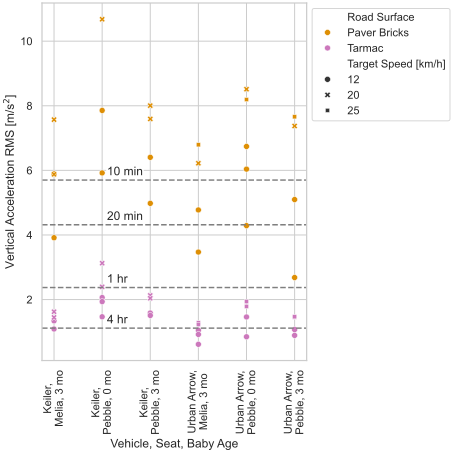
\includegraphics[width=160mm]{fig/SeatBotacc_ver-rms-bicycle-compare-all.png}
  \caption{ISO 2631-1 weighted seat pan vertical RMS acceleration of all cargo
  bicycle trials with colour representing road surface and marker style
  indicating the target speed. The horizontal grey lines with time duration
  indicators are the upper bound of the ISO 2631-1 ``health caution zone'' for
  adults seated erectly experiencing vibrations for continuous duration in a
  daily dose.}
  \label{fig:health-bicycle}
\end{figure}

For the strollers, all vibration measurements were below the health caution zone
boundary if the daily continuous exposure is less than 10~\si{\minute}.
Additionally, all vehicles pushed over tarmac were still below the zone if the
daily continuous exposure is less than 4~\si{\hour}. Pushing the Bugaboo and
Maxi-Cosi with a 0 month infant or the Stokke with a 9 month infant over
cobblestones and sidewalk slabs may have health risks if the duration exceeds
20~\si{\minute}. For almost all of the strollers pushing over any surface but
tarmac exceeded the 1~\si{\hour} risk boundary. Notably the Bugaboo and Old
Rusty with a 9 month infant fell under the 1~\si{\hour} threshold for all
surfaces. The 0 month dummy experienced worse accelerations than the 9 month
dummy in the Bugaboo and Maxi-Cosi, but that was opposite for the Stokke YOYO.
Old rusty showed the least overall acceleration magnitudes.

For both cargo bicycles the accelerations exceeded the 10~\si{\minute} health
risk threshold when ridden above 20~\si{\kilo\meter\per\hour} on paver bricks
and exceeded the 1~\si{\hour} health risk threshold when ridden more than
1~\si{\hour} above 12~\si{\kilo\meter\per\hour} on paver bricks. All but the
Keiler with the Maxi-Cosi seat and the 0 month dummy were under the 1~\si{\hour}
threshold for riding on tarmac at any target speed. Only the Urban Arrow with
the 3 month dummy is under the 4~\si{\hour} threshold when ridden at
12~\si{\kilo\meter\per\hour}. The accelerations may be less when using the
Meila Baby Shell seat versus the Maxi-Cosi car seat.

\subsection{Comfort Assessment}
%
ISO~2631-1 recommends using the magnitude of the weighted seat pan acceleration
vector for comfort assessment. Figures \ref{fig:comfort-stroller} and
\ref{fig:comfort-bicycle} plot RMS of the acceleration magnitude along with the
comfort indicators provided in the standard that are based on adults seated in
public transit for an unspecified duration.

When following the threshold definitions from the ISO~2631-1 guidelines, for the
strollers, all vehicles and surfaces are at least ``a little uncomfortable''.
The other strollers are ``fairly uncomfortable'' on tarmac. All other road
surfaces are at least ``very uncomfortable''. The Bugaboo 9 month, Green Machine
0 month over paver bricks and Old Rusty 9 month over paver bricks, sidewalk
pavers, and sidewalk slabs are ``very uncomfortable'', but all other strollers
and surfaces are ``extremely uncomfortable''.
%
\begin{figure}
  \centering
  \includegraphics[width=160mm]{fig/SeatBotacc_ver-rms-comfort-stroller-compare-all.png}
  \caption{ISO 2631-1 weighted seat pan magnitude RMS acceleration of all
  stroller repetitions with colour representing road surface. The horizontal
  brown lines with the upper bound of the ISO 2631-1 ``comfort zones'' for
  adults seated erectly experiencing vibrations in public transit.}
  \label{fig:comfort-stroller}
\end{figure}

Both of the two cargo bicycles ridden at any tested speed over paver bricks, as
well as the Keiler with the Maxi-Cosi seat over tarmac at the high speeds  fall
into the category ``extremely uncomfortable''. The other vehicle setups fall
between ``fairly uncomfortable'' and ``very uncomfortable'' over tarmac for the
range of speeds. The Urban Arrow with the Melia Baby Shell performs, on average,
the best on paver bricks and tarmac.
%
\begin{figure}
  \centering
  \includegraphics[width=160mm]{fig/SeatBotacc_ver-rms-comfort-bicycle-compare-all.png}
  \caption{ISO 2631-1 weighted seat pan magnitude RMS acceleration of all cargo
  bicycle repetitions with colour representing road surface and marker style
  representing target speed. The horizontal brown lines with the upper bound of
  the ISO 2631-1 ``comfort zones'' for adults seated erectly experiencing
  vibrations in public transit.}
  \label{fig:comfort-bicycle}
\end{figure}

\subsection{Shock test}
%
We conducted shock tests by riding the bicycle or pushing the strollers over a
square-section bump of 30x30 mm, at different speeds. The analysis focuses on
the maximum peak of the seat pan acceleration. Starting from the events' time
histories (Figure \ref{fig:shock_time-history}), we identified the peak
acceleration values for each trial, then averaged them to obtain the results
listed in Table \ref{tab:shock} for different vehicles and configurations. There
is a significant variation among tests, with the peaks for the bicycles
sometimes reaching the accelerometer's full scale (16~g). While the seat pan
accelerations for the strollers are generally lower than those experienced with
the bicycles, the configuration (0 or 9 months) may play a large role. Strollers
with the baby seat configuration for 9 months show much lower accelerations
compared to the baby cot for 0 month (Bugaboo and Maxi-Cosi). Surprisingly, the
oldest strollers (Old Rusty and Green Machine) performed very well during the
shock test, resulting in the lowest seat pan acceleration among all the tested
vehicles.
Figure \ref{fig:shock_vehicle_comparison} shows the peaks of the vertical acceleration recorded at the seat pan, grouped by different vehicles, for the shock test. As already noted in Table \ref{tab:shock}, the old strollers Old Rusty and Green Machine show lower acceleration values. We do not clearly distinguish any trend with the speed for the bicycles (``keiler'' and ``urbanarrow'').
%
\begin{figure}[ht]
  \centering
  \includegraphics[width=160mm]{fig/session015-t5-shock-bicycle-trike-maxicosi-0-SeatBotacc_ver-rep0.png}
  \caption{Raw seat pan vertical acceleration versus time from session 015: Keiler tricycle during the shock test.}
  \label{fig:shock_time-history}
\end{figure}

\begin{figure}[ht]
  \centering
  \includegraphics[width=160mm]{fig/SeatBotacc_ver-shock-test-compare.png}
  \caption{Maximum vertical acceleration recorded at the seat pan during the shock test, grouped by vehicles. The colour indicates the mean speed of the trial. The lighter the colour the lower the speed.}
  \label{fig:shock_vehicle_comparison}
\end{figure}

\begin{table}[ht]
  \centering
  \caption{Maximum seat pan acceleration [m/s²] recorded for shock test, for different vehicles and baby masses.}
  \label{tab:shock}
  \footnotesize
  \begin{tabular}{lllrrrr}
    \toprule
     & &  & Target Speed & Trial Count & Max Acceleration \\
    Vehicle Type & Model & Seat, Baby & [km/h] & & [m/s²] \\
    \midrule
    Strollers & Bugaboo & Cot, 0 mo  & 5 & 2 & 145.599 \\
              &         & Seat, 9 mo & 5 & 4 & 49.329 \\
    \cline{2-6}
              & Maxi-Cosi & Cot, 0 mo  & 5 & 2 & 131.184 \\
              &           & Seat, 9 mo & 5 & 4 & 34.941 \\
    \cline{2-6}
              & Stokke BABYZEN YOYO & Cot, 0 mo  & 5 & 4 & 34.983 \\
              &                     & Seat, 9 mo & 5 & 4 & 50.614 \\
    \cline{2-6}
              & Green Machine & Cot, 0 mo & 5 & 4 & 17.430 \\
    \cline{2-6}
              & Old Rusty & Seat, 9 mo & 5 & 4 & 31.100 \\
    \cline{1-6}
    Bicycles & Keiler tricycle & Melia, 3 mo & 5 & 2 & 52.248 \\

             &               & Melia, 3 mo & 12 & 2 & 85.209 \\

             &               & Melia, 3 mo & 20 & 2 & 123.592 \\
    \cline{2-6}
             &               & Maxi-Cosi, 0 mo & 5 & 2 & 112.755 \\

             &               & Maxi-Cosi, 0 mo & 12 & 2 & 139.623 \\

             &               & Maxi-Cosi, 0 mo & 20 & 2 & 115.345 \\
    \cline{2-6}
             &               & Maxi-Cosi, 3 mo & 5 & 2 & 151.469 \\

             &               & Maxi-Cosi, 3 mo & 12 & 2 & 160.000 \\

             &               & Maxi-Cosi, 3 mo & 20 & 2 & 145.013 \\
    \cline{2-6}
             & Urban Arrow & Melia, 3 mo & 5 & 2 & 42.742 \\

             &               & Melia, 3 mo & 12 & 2 & 42.688 \\

             &               & Melia, 3 mo & 25 & 2 & 42.3917 \\
    \cline{2-6}
             &               & Maxi-Cosi, 0 mo & 5 & 1 & 50.433 \\
    
             &               & Maxi-Cosi, 0 mo & 12 & 2 & 63.439 \\
    
             &               & Maxi-Cosi, 0 mo & 25 & 2 & 130.491 \\
    \cline{2-6}
             &               & Maxi-Cosi, 3 mo & 5 & 2 & 156.429 \\
    
             &               & Maxi-Cosi, 3 mo & 12 & 2 & 160.000 \\
    
             &               & Maxi-Cosi, 3 mo & 25 & 2 & 160.000 \\
    \bottomrule
  \end{tabular}
\end{table}


\subsection{Statistical Results}
%
Table~\ref{tab:stroller-ols} shows the results of the 11 DoF stroller model for
the 104 trials (\(R^2=0.867,F=54.69\)). Both categorical variables have
significant effects. The intercept gives the mean acceleration of the Green
Machine stroller pushed over tarmac, which is not significant. All road surfaces
cause significantly more acceleration than tarmac with cobblestones having the
largest relative effect (3.0~\si{\mps\squared} larger), followed by sidewalk
slabs (2.7~\si{\mps\squared} larger), sidewalk pavers (1.8~\si{\mps\squared}
larger), and paver bricks (1.6~\si{\mps\squared} larger). The Bugaboo, Seat, 9
mo and Maxi-Cosi, Seat, 9 mo are not significantly different than the Green
Machine, Cot, 0 mo but the other strollers are. The Old Rusty, Seat, 9 mo and
Bugaboo, Cot, 0 mo showed lower RMS acceleration than Green Machine, Cot, 0 mo
by 0.8 and 0.5~\si{\mps\squared}, respectively. The remaining strollers have
larger accelerations than the Green Machine, Cot, 0 Mo on tarmac: Maxi-Cosi,
Cot, 0 mo (1.1~\si{\mps\squared}), Bugaboo, Cot, 0 mo (1.0~\si{\mps\squared}),
YOYO, Seat, 9 mo (1.0~\si{\mps\squared}), and YOYO, Seat, 0 mo
(0.6~\si{\mps\squared}).
%
\begin{table}
  \centering
  \caption{Ordinary Linear Regression Results for Stroller. Tarmac and Green Machine Cot month are the references for the categorical Road Surface and Vehicle Setup variables.}
  \label{tab:stroller-ols}
  \footnotesize
\begin{tabular}{lcccccc}
& \textbf{coef} & \textbf{std err} & \textbf{t} & \textbf{P$> |$t$|$} & \textbf{[0.025} & \textbf{0.975]}  \\
\midrule
\textbf{Intercept}                                                                                     &       0.2212  &        0.188     &     1.177  &         0.242        &       -0.152    &        0.595     \\
Cobblestones                                     &       3.0117  &        0.163     &    18.473  &         0.000        &        2.688    &        3.336     \\
Paver Bricks                                     &       1.6000  &        0.172     &     9.299  &         0.000        &        1.258    &        1.942     \\
Sidewalk Pavers                                  &       1.7566  &        0.174     &    10.092  &         0.000        &        1.411    &        2.102     \\
Sidewalk Slabs                                   &       2.7754  &        0.167     &    16.637  &         0.000        &        2.444    &        3.107     \\
bugaboo, cot, 0 mo   &       0.9706  &        0.202     &     4.813  &         0.000        &        0.570    &        1.371     \\
bugaboo, seat, 9 mo  &      -0.5065  &        0.199     &    -2.551  &         0.012        &       -0.901    &       -0.112     \\
maxicosi, cot, 0 mo  &       1.0795  &        0.202     &     5.353  &         0.000        &        0.679    &        1.480     \\
maxicosi, seat, 9 mo &       0.3012  &        0.209     &     1.441  &         0.153        &       -0.114    &        0.716     \\
oldrusty, seat, 9 mo &      -0.7551  &        0.209     &    -3.605  &         0.001        &       -1.171    &       -0.339     \\
yoyo, cot, 0 mo]     &       0.5766  &        0.209     &     2.753  &         0.007        &        0.161    &        0.993     \\
yoyo, seat, 9 mo     &       0.9706  &        0.205     &     4.731  &         0.000        &        0.563    &        1.378     \\
\bottomrule
\end{tabular}
\end{table}

Table~\ref{tab:bicycle-ols} shows the results of the 8 DoF cargo bicycle model
for the 50 trials (\(R^2=0.925,F=63.17\)). The vehicle setup categorical variable
has significant effects, the road surface categorical variable alone does not,
but the speed and interaction of speed with road surface do have significant
effects. The intercept should theoretically be zero, because there is no
vertical vibration when the speed is zero. The intercept is not significantly
different than zero. Speed is not a significant predictor on tarmac, but the
interaction variable shows that 0.8~\si{\mps\squared} is gained in
acceleration for each 1~\si{\kph} increase on paver bricks. We see
that only the Urban Arrow with the 3 mo infant in either seat has significant
difference to the Keiler, Maxi-Cosi, 3 m, both showing reduction in relative acceleration.
%
\begin{table}
  \centering
  \caption{Ordinary Linear Regression Results for Cargo Bicycle. Tarmac and
  Keiler Maxi-Cosi 3 mo are the references for the categorical Road Surface and
  Vehicle Setup variables.}
  \label{tab:bicycle-ols}
  \footnotesize
\begin{tabular}{lcccccc}
& \textbf{coef} & \textbf{std err} & \textbf{t} & \textbf{P$> |$t$|$} & \textbf{[0.025} & \textbf{0.975]}  \\
\midrule
\textbf{Intercept}                                                                                          &       0.8067  &        0.643     &     1.255  &         0.216        &       -0.491    &        2.104     \\
Paver Bricks                                          &       1.2956  &        0.889     &     1.457  &         0.153        &       -0.500    &        3.091     \\
keiler, maxicosi, 0 mo     &       0.8664  &        0.415     &     2.085  &         0.043        &        0.027    &        1.705     \\
keiler, melia, 3 mo        &      -0.5060  &        0.415     &    -1.219  &         0.230        &       -1.344    &        0.332     \\
urbanarrow, maxicosi, 0 mo &      -0.0512  &        0.404     &    -0.127  &         0.900        &       -0.867    &        0.764     \\
urbanarrow, maxicosi, 3 mo &      -0.8895  &        0.415     &    -2.141  &         0.038        &       -1.728    &       -0.051     \\
urbanarrow, melia, 3 mo    &      -1.1357  &        0.403     &    -2.819  &         0.007        &       -1.949    &       -0.322     \\
Mean Speed [m/s]                                                                              &       0.2034  &        0.116     &     1.747  &         0.088        &       -0.032    &        0.439     \\
Mean Speed\(\times\)Road Surface                    &       0.7803  &        0.180     &     4.338  &         0.000        &        0.417    &        1.144     \\
\bottomrule
\end{tabular}
  \end{table}
  
\paragraph{Vehicle Comparisons}
%
Given that the vehicle setup is a significant effect, we can look at a posthoc
analysis to compare vehicles on each road surface.
Table~\ref{tab:sig-group-stroller}, derived from
Figure~\ref{fig:tukey-stroller}, shows the groupings of non-significant
comparisons. Old Rusty, Bugaboo with 9 month, and the Green Machine perform
generally better (significantly) that the other vehicles. For cobblestones, this
is true as well as: 1) the YOYO 9 month is the worse along with the heavier baby
performing worst than the lighter baby in the YOYO, 2) the heavier baby sees
less acceleration for the Bugaboo and Maxicosi. For paver bricks: 1) Old Rusty,
Bugaboo 9 mo, and Green Machine are the best and 2) Stokke 9 mo sees more than
the 0 mo. For sidewalk pavers, there is no significant difference among the
strollers. For side walk slabs: 1) Old Rusty is the best and Bugaboo the second
best, 2) the 0 month in the Bugaboo and Maxi-Cosi see more than the 9 month in
the same vehicle, respectively, and 3) no difference in the YOYO when comparing
baby ages. For tarmac: the Green Machine, Bugaboo 9 mo, and YOYO 9 mo are better
than Maxi-cosi with either baby age and 2) the Green Machine is better than the
Bugaboo 0 mo.
%
\begin{table}
\centering
\caption{Stroller Significance Ranking Groups (based on
Figure~\ref{fig:tukey-stroller}). The numbers indicate the group where there is
no significant difference with 1 being the best (lower acceleration) and 8 being
the worst (higher acceleration).}
\label{tab:sig-group-stroller}
\begin{tabular}{lccccc}
  \toprule
  Vehicle Setup                 & Cobblestones & Paver Bricks & Sidewalk Pavers & Sidewalk Slabs & Tarmac \\
  \midrule
  yoyo, seat, 9 mo         & 8            & 6-8          & 1-8             & 5-6            & 1-6 \\
  yoyo, cot, 0 mo          & 4-5          & 3-5          & 1-8             & 5-6            & 1-8 \\
  oldrusty, seat, 9 mo     & 1-2          & 1-3          & 1-8             & 1              & 1-8 \\
  maxicosi, seat, 9 mo     & 4-5          & 3-6          & 1-8             & 3-4            & 4-8 \\
  maxicosi, seat, 0 mo     & 6-7          & 6-8          & 1-8             & 7-8            & 4-8 \\
  greenmachine, cot, 0 mo  & 3            & 1-3          & 1-8             & 3-4            & 1-4 \\
  bugaboo, seat, 9 mo      & 1-2          & 1-3          & 1-8             & 2              & 1-6 \\
  bugaboo, cot, 0 mo       & 6-7          & 3-6          & 1-8             & 7-8            & 2-8 \\
  \bottomrule
\end{tabular}
\end{table}

When comparing the cargo bicycles, Table~\ref{tab:sig-group-bicycle}, most
vehicle setups deliver similar acceleration to the seat pan when ridden over the
same surface at the same target speed. For low speed on tarmac, the Urban Arrow
with the Meila Baby Shell and a 3 month has significantly less acceleration than
the Keiler with the Maxicosi anda 0 month baby. There is no significant
difference in any vehicle setups at low speed on paver bricks. At higher speeds,
the Urban Arrow and Kiler with the Meila seat and the 3 month is significantly
better than the Keiler with the Maxicosi and the 0 month on paver bricks and on
tarmac. It is important to point out that there is no significant difference
when simply swapping the seat for the 3 month old.
%
\begin{table}
\centering
\caption{Cargo Bicycle Significance Ranking Groups (based on
Figure~\ref{fig:tukey-bicycle}). The numbers indicate the group where there is
no significant difference with 1 being the best (lower acceleration) and 6 being
the worst (higher acceleration).}
\label{tab:sig-group-bicycle}
\begin{tabular}{lcccc}
     \toprule
                                & Paver Bricks & Tarmac    & Paver Bricks & Tarmac \\
     Vehicle Setup              & Low Speed    & Low Speed & High Speed   & High Speed \\
     \midrule
     urbanarrow, melia, 3 mo    & 1-6 & 1-5 & 1-5 & 1-5\\
     urbanarrow, maxicosi, 3 mo & 1-6 & 1-6 & 1-5 & 1-5\\
     urbanarrow, maxicosi, 0 mo & 1-6 & 1-6 & 1-6 & 1-5\\
     keiler, melia, 3 mo        & 1-6 & 1-6 & 1-5 & 1-5\\
     keiler, maxicosi, 3 mo     & 1-6 & 1-6 & 1-6 & 1-6\\
     keiler, maxicosi, 0 mo     & 1-6 & 2-6 & 3-6 & 4-6\\
     \bottomrule
\end{tabular}
\end{table}

\section{Discussion \& Conclusion}
%
We have presented a comprehensive set of acceleration measurements from
experiments that simulate the vibrations experienced by dummy infants in the 0-9
month mass range during transportation in both strollers and cargo bicycles. We
compared the average magnitude of vertical and total acceleration at the seat
pan across a variety of road surfaces and seats while moving at typical vehicle
travel speeds. ISO weighted average acceleration can range from
\SIrange{0.4}{10.7}{\mps\squared} across all tested scenarios. Strollers induced
\SIrange{0.4}{5.0}{\mps\squared} average acceleration for a mean walking speed
of 5.3~\si{\kph}. Cargo bicycles induced \SIrange{0.6}{10.7}{\mps\squared} over
a speed range of \SIrange{12}{25}{\kph}. Our investigation compared different
road surfaces, different stroller and cargo bicycle brands and types, and
different speeds for cargo bicycles.

\subsection{Surface \& Speed}
%
Travelling over a tarmac surface offers the least vibration to all vehicle types
at any speed with a maximum average acceleration of
1.2~\si{\meter\per\second\squared}. For strollers, travelling over surfaces
rougher than tarmac at normal walking speed can cause on average 5\(\times\) the
acceleration experienced on tarmac with average accelerations reaching
5.0~\si{\meter\per\second\squared}. Cobblestones and the large gaps in the
sidewalk slabs caused the largest magnitude of vibrations at the seat pan in the
strollers. Cobblestones and sidewalk slabs approximately double the vibration
amplitude relative to sidewalk paver and paver bricks, with them all being
significant larger than tarmac vibrations.

For cargo bicycles, travelling over paver bricks at the same speeds
can quadruple the magnitude of the average acceleration the dummy experiences.
Travelling at the maximum allowed speed of an electric cargo bike (25 \si{\kph})
over paver bricks caused the dummy to experience average accelerations exceeding
8~\si{\mps\squared}. The effect of speed on vibration is significant for paver
bricks but not for tarmac. Cobblestones

Whereas speed strongly affected the acceleration amplitude it does not strongly
affect the peak frequency and the bandwidth below which 80\% of power is
contained. This suggests that peak frequencies represent oscillations induced by
the systems tested rather than dominant frequencies resulting from the road
surface.

\subsection{Baby Mass}
%
The size of the dummy (mass and build) had no obvious effect on the average
acceleration at the seat pan body-seat interface. These vibrations
are transmitted to an infant's body and the physical properties (mass, stiffness,
damping) of the infant's body determine whether this excitation is amplified or
not and which body segment is more affected. Tests with more realistic
dummies or realinfants are necessary to investigate how the infant itself moves when
excited by this level of vibration. This information is not readily available in
the literature and may be hard to acquire due to ethical limitations and the
absence of validated infant dummies. The only effect that stood out for mass,
was that the lighter dummy has less acceleration than the heavier dummy for the
YOYO stroller.

\subsection{Health}
%
The vibrations measured in the different scenarios showed that average
acceleration can be relatively large when compared to the smoothest experience
on tarmac. There is a large gap in the literature connecting acceleration
magnitude to discomfort and/or health consequences, which is in particular
absent for infants. The most used health and comfort assessment tool for whole body vibration is the ISO~2631-1 standard. When we investigated health risks using the standard we found that:
%
\begin{itemize}
    \item only strollers pushed over tarmac at 5~\si{\kph} had
    average acceleration below the ``health risk zone'' for 4~\si{\hour} daily
    duration
    \item strollers pushed over cobblestones and pavers can deliver
    accelerations in the health risk zone with durations as short as
    20~\si{\min}
    \item cargo bicycles ridden at \SIrange{12}{25}{\kph} over tarmac
    overwhelmingly delivered accelerations below the 1~\si{\hour} ``health risk
    zone''
    \item cargo bicycles ridden at \SIrange{12}{25}{\kph} over paver bricks
    delivered accelerations well into the 10~\si{\min} ``health risk zone''
\end{itemize}
%
We can conclude that strollers should be pushed slower than 5~\si{\kph} over
non-tarmac road surfaces and for continuous durations less than 10~\si{\min}.
Cargo bicycles carrying infants should slow down less than 12~\si{\min} over
paver bricks and/or the duration should be kept under 10~\si{\min}. When riding
a cargo bicycle over tarmac durations should be kept under 1~\si{\hour}.

\subsection{Comfort}
%
When considering comfort, the ISO~2631-1 guidelines indicate that adults would
report the vibrations experienced in strollers and bicycles as uncomfortable.
For strollers, the vibrations over tarmac would be rated ``fairly
uncomfortable'' and all other road surfaces would be ``very'' or ``extremely
uncomfortable''. When riding a cargo bicycle over paver bricks, the vibrations
would be rated as ``extremely uncomfortable'' and over tarmac spans ``fairly``
to ``extremely''. The ISO comfort rating scale is derived from adult subjective
ratings of vibrations felt when riding public transit for an unspecified
duration, so this scale is unlikely appropriate to apply for our situation.
Gao~\cite{gao2018} reports that cyclists do not rate vibrations as extremely
uncomfortable on normal road surfaces, so that indicates some contradiction.

\subsection{Vehicle \& Seat Design}
%
Different vehicle, seat, and baby mass combinations cause different average
vertical acceleration at the seat pan. A striking discovery is that the two
1970's strollers we tested were significantly better than many of the modern
stroller setups on most road surfaces. The old strollers actually had more
sophisticated suspension systems that utilized springs, straps, and mechanisms
and they also had larger wheels. Road surfaces have gotten smoother over the
last two centuries and stroller manufacturers may have reduced the efforts in
suspension design as a side effect. The ``Old Rusty'' stroller was the only one
that did not exceed the 1~\si{\hour} health risk line for all road surfaces.

Both the Bugaboo and Maxi-Cosi stroller showed lower acceleration for the
heavier baby, as expected, but the Stokke YOYO showed the opposite trend for
cobblestones and paver bricks. This points to design choices that may cause
resonance on certain surface profiles. The Bugaboo in the 9 mo seat
configuration performed better than the other modern strollers for all
non-tarmac road surfaces.

Urban Arrow better than Keiler on tarmac but there is no difference on paver
bricks. Additionally, there was no difference in the different seats for the 3
month infant.

\subsection{ISO Filters and Bandwidth}
%
Vibrations at frequencies between
\SIrange{4.9}{10.7}{\hertz} showed to have the largest magnitude contribution to the
vibrations, but there is a frequency content of magnitudes of interest in a
bandwidth of up to 45~\si{\hertz}.

We report root mean squared (RMS) accelerations up to 120 Hz as well as accelerations weighted according to the ISO norms for vibration (VDV). Our results show substantial differences between RMS and VDV highlighting the importance of reviewing their meaning. These differences emerge from the high bandwidth of the accelerations now measured, which greatly exceed the bandwidth of accelerations measured with adults seated in cars (see e.g Figure 2 in \cite{griffin2004experimental}). Adult experiments show that significant discomfort can be measured across all tested frequencies being 80 Hz \cite{morioka2010frequency} or even 315 Hz \cite{morioka2006magnitude} albeit with reduced sensitivity.
The ISO frequency weightings are defined for adults in more or less erect postures with the head being unsupported, whereas we now studied dummies representing infants from 0 - 9 months lying with the head directly supported. The ISO weightings represent a reduced sensitivity above 8 Hz, which is associated by the vertical dynamics of erect seated subjects which filter out such high frequencies [add ref]. However, adult experiments show higher discomfort for frequencies above 8 Hz when lying with head supported with 30-90 deg back inclination as compared to erect without head support.
Higher frequencies have also been associated with effects on the central nervous system. For instance, experiments on rats showed brain injury visible in behaviour through functional impairment and in visual changes of brain structures in postmortem dissection after exposure to prolonged whole-body vibration at 30 Hz and 0.5 G \cite{Yan2015_cumulative_brain_injury/j.jstrokecerebrovasdis.2015.08.007}.
In some conditions the RMS exceeds the ISO based VDV by a factor [add number], warranting further research on the effects of higher frequencies in particular for head supported conditions and for children.

\subsection{Summary, Recommendations, and Future Work}
%
The results herein raise concerns about transporting infants in strollers and
cargo bicycles. If the pusher or rider's behavior is not adjusted to avoid rough
surfaces or to go very slow over them when the cargo is an infant, there are
potential health risks if the large vibrations are experienced daily and
repeatedly  for years. In most likelihood parents do adjust their travel
behavior but maybe not enough or they are neglectful but this has yet to be
studied. There is not direct evidence that connects whole body vibration as
measured in this study to infant harm or negative health effects, so we can only
extroplate from the limited guidelines on adults in occupational settings. But
we did measure vibrations that would not be permitted for adults to maintain
occuptaionl health and it is reasonble to beleive we should nto subject our
infants to the same. It is well known that whole body vibration can be
controlled with good suspension design. We see this in the drastic evolution of
suspension in automobiles. We do not see this same kind of attention for
suspsension in strollers, cargo bicycles, and baby seats for these vehicles.
Increasing walking and cycling is well known to offer great societal and
personal benefits over traveling with automoble, so it behoves us all to make
transport for infants most optimal in these two transport modes. The following
list provides recommendations for parents, researchers, and manufacturers based on the findings of this paper:
%
\begin{itemize}
    \item Stroller, Cargo Bicycle, and Seat manufacturers must test for
    vibration magnitude and frequency over all expected surface types to ensure
    their designs dampened vibrations well for all scenarios.
    \item Need to design better suspension systems, as vibrations can be
    drastically reduced. Looking to past designs when road surfaces were not so
    smooth is pertinent.
    \item Parents should push or ride slowly over surfaces rougher than tarmac,
    as bumpier surfaces can quickly multiply the experience acceleration.
    \item Parents should limit the duration of transport over surfaces rougher
    than tarmac periods that do not exceed 10 minutes with adequate
    non-vibration breaks in between. When transporting over tarmac, durations should not exceed 4 hours.
    \item E-cargo bicycles can easily reach the maximum speed of 25~\si{\kph}
    and infants should be transported for long durations when riding over
    non-tarmac surfaces at these speeds.
    \item ISO 2631-1 is not adequate for accurately characterizing health and
    comfort for infants or children or for short durations or non-erect seating.
    Research is needed to develop a new standard for assessing whole body
    vibration of infants and children.
\end{itemize}

We acquired data from four other sensors on the vehicles, all with three
accelerometer and three gyroscope time histories, for a total of 30 time
histories of possible interest. This paper provides a look into the experiments
via three metrics: ISO weighted vertical RMS acceleration, peak frequency, and
bandwidth of the seat pan sensor. The collected data can also be used to
investigate transmissibility from sensor to sensor as well as rotational
vibration effects. Investigating these further can give a more complete picture
of the connections to health and comfort. This work also gives a benchmark that
new designs can be tested against so show reduction in vibration.

\bibliographystyle{plain}
\bibliography{reference}

\newpage
\appendix

% Ensure subsections retain "A.1", "A.2", etc.
%\addcontentsline{toc}{section}{Appendix} % Optional: Add to TOC
%\renewcommand{\thesection}{A}
%\renewcommand{\thesubsection}{\thesection.\arabic{subsection}}

\section{All Trial Metrics}
%
Table~\ref{tab:results} shows the mean over the scenario trials unweighted and
ISO~2631-1 weighted seat pan vertical RMS acceleration, duration, peak
frequency, bandwidth, and crest factor for all 52 combinations of vehicle setup,
road surface, and target speed.
% NOTE : This table is generated automatically from the Python scripts. I manually edit the header rows to fit on the page width. Save the edits between toprule and midrule!
\bgroup
\setlength\tabcolsep{0.8mm}  % reduces horiztonal padding between columns
\begin{table}
  \centering
  \caption{Mean computed metrics for all 52 scenarios.}
  \label{tab:results}
  \footnotesize
\begin{tabular}{lllcccccccc}
\toprule
& & & Target & Trial & RMS & Weighted & Peak & & & Crest \\
& & Road & Speed & Count & Accel & RMS Accel & Frequency & Bandwidth & Duration  & Factor \\
Vehicle & Seat, Baby & Surface & [km/h] & & [m/s/s] & [m/s/s] & [Hz] & [Hz] & [s]  & \\
\midrule
\multirow[t]{10}{*}{bugaboo} & \multirow[t]{5}{*}{cot, 0 mo} & Cobblestones & 5 & 4 & 4.4 & 4.3 & 6.5 & 14.3 & 20.4 & 6.2 \\
\cline{3-11}
 &  & Paver Bricks & 5 & 3 & 2.6 & 2.4 & 9.5 & 17.2 & 23.3 & 4.1 \\
\cline{3-11}
 &  & Sidewalk Pavers & 5 & 2 & 2.9 & 2.7 & 6.1 & 18.5 & 25.4 & 13.5 \\
\cline{3-11}
 &  & Sidewalk Slabs & 5 & 3 & 4.8 & 4.7 & 5.8 & 15.1 & 20.2 & 6.4 \\
\cline{3-11}
 &  & Tarmac & 5 & 2 & 0.7 & 0.6 & 10.1 & 18.5 & 23.1 & 3.3 \\
\cline{2-11} \cline{3-11}
 & \multirow[t]{5}{*}{seat, 9 mo} & Cobblestones & 5 & 4 & 2.5 & 2.3 & 6.6 & 20.7 & 22.5 & 4.7 \\
\cline{3-11}
 &  & Paver Bricks & 5 & 3 & 2.3 & 1.8 & 9.4 & 26.4 & 22.6 & 3.8 \\
\cline{3-11}
 &  & Sidewalk Pavers & 5 & 3 & 1.7 & 1.4 & 7.7 & 23.8 & 24.7 & 5.5 \\
\cline{3-11}
 &  & Sidewalk Slabs & 5 & 3 & 2.4 & 2.2 & 6.0 & 20.3 & 24.5 & 5.3 \\
\cline{3-11}
 &  & Tarmac & 5 & 2 & 0.6 & 0.4 & 8.4 & 29.3 & 34.6 & 6.5 \\
\cline{1-11} \cline{2-11} \cline{3-11}
\multirow[t]{5}{*}{greenmachine} & \multirow[t]{5}{*}{cot, 0 mo} & Cobblestones & 5 & 3 & 3.2 & 2.9 & 4.1 & 17.3 & 23.7 & 5.3 \\
\cline{3-11}
 &  & Paver Bricks & 5 & 2 & 1.6 & 1.3 & 4.2 & 26.8 & 29.6 & 4.5 \\
\cline{3-11}
 &  & Sidewalk Pavers & 5 & 2 & 2.7 & 2.5 & 4.1 & 18.5 & 28.2 & 6.5 \\
\cline{3-11}
 &  & Sidewalk Slabs & 5 & 3 & 3.5 & 3.2 & 3.9 & 16.8 & 23.9 & 6.7 \\
\cline{3-11}
 &  & Tarmac & 5 & 2 & 0.5 & 0.4 & 4.2 & 33.4 & 22.1 & 4.1 \\
\cline{1-11} \cline{2-11} \cline{3-11}
\multirow[t]{12}{*}{keiler} & \multirow[t]{4}{*}{maxicosi, 0 mo} & \multirow[t]{2}{*}{Paver Bricks} & 12 & 2 & 7.0 & 6.9 & 7.6 & 16.7 & 23.8 & 7.2 \\
 &  &  & 20 & 1 & 12.6 & 10.7 & 6.8 & 26.9 & 34.0 & 9.9 \\
\cline{3-11}
 &  & \multirow[t]{2}{*}{Tarmac} & 12 & 3 & 1.8 & 1.8 & 8.1 & 13.3 & 24.6 & 8.3 \\
 &  &  & 20 & 2 & 2.8 & 2.8 & 7.8 & 13.2 & 29.2 & 5.1 \\
\cline{2-11} \cline{3-11}
 & \multirow[t]{4}{*}{maxicosi, 3 mo} & \multirow[t]{2}{*}{Paver Bricks} & 12 & 2 & 6.3 & 5.7 & 8.0 & 21.9 & 28.9 & 11.0 \\
 &  &  & 20 & 2 & 9.8 & 7.8 & 7.2 & 30.7 & 21.4 & 14.4 \\
\cline{3-11}
 &  & \multirow[t]{2}{*}{Tarmac} & 12 & 2 & 1.5 & 1.5 & 7.6 & 12.8 & 27.8 & 8.1 \\
 &  &  & 20 & 2 & 2.1 & 2.1 & 6.4 & 12.7 & 23.8 & 3.9 \\
\cline{2-11} \cline{3-11}
 & \multirow[t]{4}{*}{melia, 3 mo} & \multirow[t]{2}{*}{Paver Bricks} & 12 & 2 & 5.4 & 4.9 & 7.9 & 21.9 & 26.3 & 8.1 \\
 &  &  & 20 & 2 & 9.5 & 6.7 & 6.8 & 34.8 & 23.0 & 10.2 \\
\cline{3-11}
 &  & \multirow[t]{2}{*}{Tarmac} & 12 & 2 & 1.2 & 1.2 & 7.8 & 14.2 & 25.4 & 8.2 \\
 &  &  & 20 & 2 & 1.6 & 1.5 & 8.3 & 13.8 & 22.6 & 3.8 \\
\cline{1-11} \cline{2-11} \cline{3-11}
\multirow[t]{10}{*}{maxicosi} & \multirow[t]{5}{*}{cot, 0 mo} & Cobblestones & 5 & 4 & 4.6 & 4.4 & 8.1 & 18.3 & 20.7 & 4.9 \\
\cline{3-11}
 &  & Paver Bricks & 5 & 2 & 3.2 & 2.8 & 10.4 & 21.1 & 27.2 & 3.9 \\
\cline{3-11}
 &  & Sidewalk Pavers & 5 & 3 & 3.0 & 2.9 & 7.6 & 18.1 & 21.4 & 5.5 \\
\cline{3-11}
 &  & Sidewalk Slabs & 5 & 3 & 5.0 & 4.6 & 5.1 & 20.7 & 16.3 & 8.2 \\
\cline{3-11}
 &  & Tarmac & 5 & 2 & 0.9 & 0.8 & 9.6 & 24.4 & 34.3 & 8.0 \\
\cline{2-11} \cline{3-11}
 & \multirow[t]{5}{*}{seat, 9 mo} & Cobblestones & 5 & 3 & 4.1 & 3.7 & 8.0 & 20.3 & 25.9 & 5.8 \\
\cline{3-11}
 &  & Paver Bricks & 5 & 2 & 3.0 & 2.4 & 9.7 & 24.0 & 27.8 & 3.4 \\
\cline{3-11}
 &  & Sidewalk Pavers & 5 & 2 & 2.6 & 2.3 & 7.3 & 21.2 & 27.8 & 5.5 \\
\cline{3-11}
 &  & Sidewalk Slabs & 5 & 3 & 3.1 & 2.9 & 6.9 & 20.1 & 25.6 & 5.4 \\
\cline{3-11}
 &  & Tarmac & 5 & 2 & 1.0 & 0.7 & 10.2 & 30.0 & 36.1 & 5.8 \\
\cline{1-11} \cline{2-11} \cline{3-11}
\multirow[t]{5}{*}{oldrusty} & \multirow[t]{5}{*}{seat, 9 mo} & Cobblestones & 5 & 2 & 4.7 & 2.0 & 5.1 & 39.0 & 29.9 & 6.0 \\
\cline{3-11}
 &  & Paver Bricks & 5 & 3 & 3.4 & 1.2 & 5.2 & 44.2 & 21.9 & 6.1 \\
\cline{3-11}
 &  & Sidewalk Pavers & 5 & 2 & 3.3 & 1.4 & 5.4 & 40.1 & 27.3 & 9.7 \\
\cline{3-11}
 &  & Sidewalk Slabs & 5 & 3 & 3.2 & 1.6 & 5.3 & 39.0 & 23.8 & 11.6 \\
\cline{3-11}
 &  & Tarmac & 5 & 2 & 1.1 & 0.5 & 7.0 & 42.1 & 22.6 & 5.7 \\
\cline{1-11} \cline{2-11} \cline{3-11}
\multirow[t]{15}{*}{urbanarrow} & \multirow[t]{5}{*}{maxicosi, 0 mo} & \multirow[t]{3}{*}{Paver Bricks} & 12 & 3 & 6.5 & 5.7 & 7.6 & 21.4 & 20.8 & 9.6 \\
 &  &  & 20 & 1 & 9.2 & 8.5 & 8.0 & 19.8 & 39.1 & 9.9 \\
 &  &  & 25 & 1 & 11.6 & 8.2 & 6.9 & 38.0 & 38.3 & 13.7 \\
\cline{3-11}
 &  & \multirow[t]{2}{*}{Tarmac} & 12 & 2 & 1.3 & 1.2 & 9.3 & 18.5 & 29.0 & 8.3 \\
 &  &  & 25 & 2 & 2.1 & 1.9 & 9.7 & 18.1 & 21.5 & 5.2 \\
\cline{2-11} \cline{3-11}
 & \multirow[t]{5}{*}{maxicosi, 3 mo} & \multirow[t]{3}{*}{Paver Bricks} & 12 & 2 & 4.5 & 3.9 & 5.8 & 21.6 & 29.1 & 13.5 \\
 &  &  & 20 & 1 & 10.8 & 7.4 & 5.0 & 32.4 & 32.1 & 14.7 \\
 &  &  & 25 & 1 & 10.6 & 7.7 & 6.3 & 31.2 & 30.3 & 14.7 \\
\cline{3-11}
 &  & \multirow[t]{2}{*}{Tarmac} & 12 & 2 & 1.1 & 1.0 & 8.8 & 18.3 & 25.3 & 9.6 \\
 &  &  & 25 & 2 & 1.6 & 1.5 & 9.5 & 18.3 & 21.6 & 4.9 \\
\cline{2-11} \cline{3-11}
 & \multirow[t]{5}{*}{melia, 3 mo} & \multirow[t]{3}{*}{Paver Bricks} & 12 & 2 & 4.5 & 4.1 & 7.5 & 18.9 & 24.1 & 8.3 \\
 &  &  & 20 & 1 & 6.9 & 6.2 & 7.9 & 21.2 & 36.8 & 8.6 \\
 &  &  & 25 & 1 & 7.6 & 6.8 & 9.2 & 21.1 & 31.7 & 7.2 \\
\cline{3-11}
 &  & \multirow[t]{2}{*}{Tarmac} & 12 & 3 & 0.9 & 0.9 & 9.4 & 16.7 & 20.4 & 9.3 \\
 &  &  & 25 & 2 & 1.4 & 1.3 & 9.4 & 16.6 & 23.0 & 5.8 \\
\cline{1-11} \cline{2-11} \cline{3-11}
\multirow[t]{10}{*}{yoyo} & \multirow[t]{5}{*}{cot, 0 mo} & Cobblestones & 5 & 3 & 4.1 & 4.0 & 6.4 & 16.9 & 21.3 & 4.8 \\
\cline{3-11}
 &  & Paver Bricks & 5 & 2 & 3.0 & 2.1 & 9.4 & 41.7 & 29.5 & 4.1 \\
\cline{3-11}
 &  & Sidewalk Pavers & 5 & 3 & 2.8 & 2.6 & 6.7 & 18.8 & 22.2 & 5.5 \\
\cline{3-11}
 &  & Sidewalk Slabs & 5 & 2 & 4.0 & 3.8 & 5.2 & 19.6 & 25.7 & 6.4 \\
\cline{3-11}
 &  & Tarmac & 5 & 2 & 0.9 & 0.6 & 7.7 & 42.9 & 19.5 & 7.4 \\
\cline{2-11} \cline{3-11}
 & \multirow[t]{5}{*}{seat, 9 mo} & Cobblestones & 5 & 3 & 5.2 & 4.9 & 7.7 & 17.6 & 21.5 & 4.4 \\
\cline{3-11}
 &  & Paver Bricks & 5 & 3 & 3.6 & 3.0 & 10.4 & 25.0 & 22.5 & 3.8 \\
\cline{3-11}
 &  & Sidewalk Pavers & 5 & 2 & 3.1 & 2.7 & 8.3 & 23.4 & 28.5 & 9.9 \\
\cline{3-11}
 &  & Sidewalk Slabs & 5 & 3 & 4.0 & 3.7 & 5.3 & 19.0 & 23.3 & 6.2 \\
\cline{3-11}
 &  & Tarmac & 5 & 2 & 0.7 & 0.4 & 11.1 & 41.7 & 39.1 & 6.3 \\
\cline{1-11} \cline{2-11} \cline{3-11}
\bottomrule
\end{tabular}
\end{table}
\egroup
\section{Vehicle Statistical Comparisons}
%
\begin{figure}[!h]
  \centering
  \subcaptionbox{}{
  \includegraphics[width=75mm]{fig/tukey-SeatBotacc_ver-stroller-Cobblestones.png}}
  \subcaptionbox{}{
  \includegraphics[width=75mm]{fig/tukey-SeatBotacc_ver-stroller-Paver Bricks.png}}
  \subcaptionbox{}{
  \includegraphics[width=75mm]{fig/tukey-SeatBotacc_ver-stroller-Sidewalk Pavers.png}}
  \subcaptionbox{}{
  \includegraphics[width=75mm]{fig/tukey-SeatBotacc_ver-stroller-Sidewalk Slabs.png}}
  \subcaptionbox{}{
  \includegraphics[width=75mm]{fig/tukey-SeatBotacc_ver-stroller-Tarmac.png}}
  \caption{Tukey Comparison Plots for the Strollers}
  \label{fig:tukey-stroller}
\end{figure}
%
\begin{figure}[!h]
  \centering
  \subcaptionbox{}{
  \includegraphics[width=75mm]{fig/tukey-SeatBotacc_ver-bicycle-Paver Bricks-Low.png}}
  \subcaptionbox{}{
  \includegraphics[width=75mm]{fig/tukey-SeatBotacc_ver-bicycle-Tarmac-Low.png}}
  \subcaptionbox{}{
  \includegraphics[width=75mm]{fig/tukey-SeatBotacc_ver-bicycle-Paver Bricks-High.png}}
  \subcaptionbox{}{
  \includegraphics[width=75mm]{fig/tukey-SeatBotacc_ver-bicycle-Tarmac-High.png}}
  \caption{Tukey Comparison Plots for the Cargo Bicycles}
  \label{fig:tukey-bicycle}
\end{figure}

\section{Experimental Equipment}
\label{app:equipment}
%
In this section, we report the pictures of the strollers and bicycles used for
the experiments. The reader can find the measurements, wheelbase, wheel
diameter, sensor location and orientation for all the tested vehicles.

\begin{figure}[htbp]    % use [htbp] to place the figures where I prefer
  \centering
  \subcaptionbox{Lateral view}{\includegraphics[width=75mm]{fig/TechDraw_UA-Joolz_lat.PNG}}
  \subcaptionbox{Front view}{\includegraphics[width=75mm]{fig/TechDraw_UA-Joolz_front.PNG}}
  \caption{IMU locations on the Urban Arrow cargo bicycle, equipped with the
  Maxicosi-Joolz baby pebble.}
  \label{fig:tech_drawing_UA_Joolz}
\end{figure}

\begin{figure}[htbp]    % use [htbp] to place the figures where I prefer
  \centering
  \subcaptionbox{Lateral view}{\includegraphics[width=75mm]{fig/TechDraw_UA-Melia_lat.PNG}}
  \subcaptionbox{Front view}{\includegraphics[width=75mm]{fig/TechDraw_UA-Melia_front.PNG}}
  \caption{IMU locations on the Urban Arrow cargo bicycle, equipped with the
  Melia baby shell.}
  \label{fig:tech_drawing_UA_Melia}
\end{figure}

\clearpage
\begin{figure}[htbp]
  \centering
  \subcaptionbox{Lateral view}{\includegraphics[width=75mm]{fig/TechDraw_Trike-Joolz_lat.PNG}}
  \subcaptionbox{Front view}{\includegraphics[width=75mm]{fig/TechDraw_Trike-Joolz_front.PNG}}
  \caption{IMU locations on the Keiler Tricycle, equipped with the
  Maxicosi-Joolz baby pebble.}
  \label{fig:tech_drawing_Trike_Joolz}
\end{figure}


\begin{figure}[htbp]
  \centering
  \subcaptionbox{Lateral view}{\includegraphics[width=75mm]{fig/TechDraw_Trike-Melia_lat.PNG}}
  \subcaptionbox{Front view}{\includegraphics[width=75mm]{fig/TechDraw_Trike-Melia_front.PNG}}
  \caption{IMU locations on the Keiler Tricycle, equipped with the
  Melia baby shell.}
  \label{fig:tech_drawing_Trike_Melia}
\end{figure}

\clearpage
\begin{figure}[htbp]
  \centering
  \subcaptionbox{Lateral view}{\includegraphics[width=70mm]{fig/TechDraw_Bugaboo0_lat.PNG}}
  \subcaptionbox{Front view}{\includegraphics[width=70mm]{fig/TechDraw_Bugaboo0_front.PNG}}
  \caption{IMU locations on the stroller Bugaboo Fox 5, configured for 0-months baby.}
  \label{fig:tech_drawing_Bugaboo0}
\end{figure}

\begin{figure}[htbp]
  \centering
  \subcaptionbox{Lateral view}{\includegraphics[width=70mm]{fig/TechDraw_Bugaboo9_lat.PNG}}
  \subcaptionbox{Front view}{\includegraphics[width=70mm]{fig/TechDraw_Bugaboo9_front.PNG}}
  \caption{IMU locations on the stroller Bugaboo Fox 5, configured for 9-months baby.}
  \label{fig:tech_drawing_Bugaboo9}
\end{figure}

\clearpage
\begin{figure}[htbp]
  \centering
  \subcaptionbox{Lateral view}{\includegraphics[width=70mm]{fig/TechDraw_Maxicosi0_lat.PNG}}
  \subcaptionbox{Front view}{\includegraphics[width=70mm]{fig/TechDraw_Maxicosi0_front.PNG}}
  \caption{IMU locations on the stroller Maxi-cosi Street +, configured for 0-months baby.}
  \label{fig:tech_drawing_Maxicosi0}
\end{figure}

\begin{figure}[htbp]
  \centering
  \subcaptionbox{Lateral view}{\includegraphics[width=70mm]{fig/TechDraw_Maxicosi9_lat.PNG}}
  \subcaptionbox{Front view}{\includegraphics[width=70mm]{fig/TechDraw_Maxicosi9_front.PNG}}
  \caption{IMU locations on the stroller Maxi-cosi Street +, configured for 9-months baby.}
  \label{fig:tech_drawing_Maxicosi9}
\end{figure}

\clearpage
\begin{figure}[htbp]
  \centering
  \subcaptionbox{Lateral view}{\includegraphics[width=70mm]{fig/TechDraw_YOYO0_lat.PNG}}
  \subcaptionbox{Front view}{\includegraphics[width=70mm]{fig/TechDraw_YOYO0_front.PNG}}
  \caption{IMU locations on the stroller Stokke YOYO, configured for 0-months baby.}
  \label{fig:tech_drawing_YOYO0}
\end{figure}

\begin{figure}[htbp]
  \centering
  \subcaptionbox{Lateral view}{\includegraphics[width=70mm]{fig/TechDraw_YOYO9_lat.PNG}}
  \subcaptionbox{Front view}{\includegraphics[width=70mm]{fig/TechDraw_YOYO9_front.PNG}}
  \caption{IMU locations on the stroller Stokke YOYO, configured for 9-months baby.}
  \label{fig:tech_drawing_YOYO9}
\end{figure}

\clearpage
\begin{figure}[htbp]
  \centering
  \subcaptionbox{Lateral view}{\includegraphics[width=70mm]{fig/TechDraw_GreenM0_lat.PNG}}
  \subcaptionbox{Front view}{\includegraphics[width=70mm]{fig/TechDraw_GreenM0_front.PNG}}
  \caption{IMU locations on the old stroller GreenMachine, configured for 0-months baby.}
  \label{fig:tech_drawing_GreenM0}
\end{figure}

\begin{figure}[htbp]
  \centering
  \subcaptionbox{Lateral view}{\includegraphics[width=70mm]{fig/TechDraw_OldR9_lat.PNG}}
  \subcaptionbox{Front view}{\includegraphics[width=70mm]{fig/TechDraw_OldR9_front.PNG}}
  \caption{IMU locations on the old stroller OldRusty, configured for 9-months baby.}
  \label{fig:tech_drawing_OldR9}
\end{figure}

\clearpage
\newpage

\subsection{Location and pictures of the experiment areas}

\subsubsection{For Bicycles}

\begin{itemize}
    \item Tarmac
\begin{figure}[htbp]
  \centering
  \subcaptionbox{Tarmac surface where we tested bicycles}{\includegraphics[width=70mm, angle=-90]{fig/Tarmac_bicycle.jpg}}
  \subcaptionbox{Satellite view from Google Maps, with the GPS coordinates}{\includegraphics[width=70mm]{fig/Tarmac_bicycle_GPS.PNG}}
  \caption{Details of the tarmac test area.}
  \label{fig:tarmac_bicycle}
\end{figure}

The bicycle experiment on the tarmac was conducted along Leeghwaterstraat, 2628 CA Delft, The Netherlands.

    \item Paver bricks
\begin{figure}[htbp]
  \centering
  \subcaptionbox{Paver bricks surface where we tested bicycles}{\includegraphics[width=70mm, angle=-90]{fig/Paver_bricks_bicycle.jpg}}
  \subcaptionbox{Satellite view from Google Maps, with the GPS coordinates}{\includegraphics[width=70mm]{fig/Paver_bricks_bicycle_GPS.PNG}}
  \caption{Details of the paver bricks test area.}
  \label{fig:paver_bricks_bicycle}
\end{figure}

The bicycle experiment on the paver bricks was conducted along Leeghwaterstraat, 2628 CA Delft, The Netherlands.

\clearpage

    \item Shock

\begin{figure}[htbp]
  \centering
  \subcaptionbox{We performed a shock test with bicycles riding over a 30x30 mm square section bar}{\includegraphics[width=70mm, angle=0]{fig/Shock_bicycle.PNG}}
  \subcaptionbox{Satellite view from Google Maps, with the GPS coordinates}{\includegraphics[width=70mm]{fig/Tarmac_bicycle_GPS.PNG}}
  \caption{Details of the shock test area.}
  \label{fig:shock_bicycle}
\end{figure}

The bicycle shock experiment was conducted along Leeghwaterstraat, 2628 CA Delft, The Netherlands (same location of the experiment on the tarmac).
Details of the shock experiment: we rode over a squared section aluminium bar 30 x 30 mm.

\end{itemize}

\subsubsection{For Strollers}

\begin{itemize}
    \item Tarmac

\begin{figure}[htbp]
  \centering
  \subcaptionbox{Tarmac surface where we tested strollers}{\includegraphics[width=70mm, angle=-90]{fig/Tarmac_stroller.jpg}}
  \subcaptionbox{Satellite view from Google Maps, with the GPS coordinates}{\includegraphics[width=70mm]{fig/Tarmac_stroller_GPS.PNG}}
  \caption{Details of the tarmac test area.}
  \label{fig:tarmac_stroller}
\end{figure}

The bicycle experiment on the tarmac was conducted along Julianalaan Straat, 2628 BG Delft, The Netherlands.

\clearpage

    \item Cobblestone

\begin{figure}[htbp]
  \centering
  \subcaptionbox{Cobblestone surface where we tested strollers}{\includegraphics[width=60mm, angle=0]{fig/Cobblestone_stroller.PNG}}
  \subcaptionbox{Satellite view from Google Maps, with the GPS coordinates}{\includegraphics[width=70mm]{fig/Tarmac_stroller_GPS.PNG}}
  \caption{Details of the cobblestone test area.}
  \label{fig:cobblestone_area_stroller}
\end{figure}

The bicycle experiment on the cobblestone was conducted along Julianalaan Straat, 2628 BG Delft, The Netherlands.
Details of cobblestone: rectangular shape, dimensions 180 x 125 mm (gap in between: 20±4 mm).

    \item Sidewalk pavers

\begin{figure}[htbp]
  \centering
  \subcaptionbox{Sidewalk pavers where we tested strollers}{\includegraphics[width=60mm, angle=0]{fig/Sidewalk_pavers_stroller.PNG}}
  \subcaptionbox{Satellite view from Google Maps, with the GPS coordinates}{\includegraphics[width=70mm]{fig/Paver_bricks_stroller_GPS.PNG}}
  \caption{Details of the sidewalk pavers test area.}
  \label{fig:sidewalkpavers_area_stroller}
\end{figure}

The experiment was conducted along Prins Bernhardlaan, 2628 CN Delft, The Netherlands (same location as Paver bricks test).
Details of sidewalk bricks: rectangular shape, dimensions 290 x 290 mm (gap in between: 12±2 mm).

\clearpage

    \item Sidewalk slabs

\begin{figure}[htbp]
  \centering
  \subcaptionbox{Sidewalk slabs where we tested strollers}{\includegraphics[width=70mm, angle=-90]{fig/Sidewalk_slabs_stroller.jpg}}
  \subcaptionbox{Satellite view from Google Maps, with the GPS coordinates}{\includegraphics[width=70mm]{fig/Sidewalk_slabs_stroller_GPS.PNG}}
  \caption{Details of the sidewalk slab test area.}
  \label{fig:sidewalkslabs_area_stroller}
\end{figure}

The experiment was conducted in front of TU Delft Aula Conference Centre (Building 20), Mekelweg 5, 2628 CC Delft, The Netherlands.
Details of sidewalk slab: made of concrete, rectangular shape, dimensions 2000 x 990 mm (gap in between: 160±3 mm).

    \item Paver bricks

\begin{figure}[htbp]
  \centering
  \subcaptionbox{Paver bricks area where we tested strollers}{\includegraphics[width=50mm, angle=0]{fig/Paver_bricks_stroller.PNG}}
  \subcaptionbox{Satellite view from Google Maps, with the GPS coordinates}{\includegraphics[width=70mm]{fig/Sidewalk_slabs_stroller_GPS.PNG}}
  \caption{Details of the paver bricks test area.}
  \label{fig:paverbrick_area_stroller}
\end{figure}

The experiment was conducted along Prins Bernhardlaan, 2628 CN Delft, The Netherlands (same location as Sidewalk bricks test).
Details of paver brick: rectangular shape, dimensions 195 x 95 mm (gap in between: 7±2 mm).

\clearpage

    \item Shock

\begin{figure}[htbp]
  \centering
  \subcaptionbox{Area where we tested strollers during the shock experiment.}{\includegraphics[width=60mm, angle=-90]{fig/Shock_stroller.jpg}}
  \subcaptionbox{Satellite view from Google Maps, with the GPS coordinates}{\includegraphics[width=70mm]{fig/Shock_stroller_GPS.PNG}}
  \caption{Details of the shock test area.}
  \label{fig:shock_area_stroller}
\end{figure}

The experiment was conducted inside TU Delft Mechanical Engineering faculty (Building 34 - Ground floor, aisle in front of Gezelschap Leeghwater office), Mekelweg 2, 2628 CD Delft, The Netherlands
Details of the shock experiment: we pushed the stroller over a squared section aluminium bar 30 x 30 mm.

\end{itemize}

\end{document}

